\documentclass[11pt]{article}
\usepackage{graphicx}
\usepackage{float}
\usepackage{caption}
\usepackage{subcaption}
\usepackage{geometry}
\geometry{a4paper, margin=1in}
\usepackage{amsmath, amsfonts, amssymb}
\usepackage{booktabs, array}
\usepackage{fancyhdr}
\usepackage{titlesec}
\usepackage{listings}
\usepackage{xcolor}
\usepackage[hidelinks]{hyperref}
\usepackage{enumitem}
\usepackage{cite}
\usepackage{listings}
\usepackage{subcaption}
\usepackage{url}
\usepackage{hyperref}
\usepackage[T1]{fontenc}
\usepackage[scaled]{beramono} % optional: better monospace font
\usepackage{subcaption} % Make sure you have this package loaded
\usepackage{caption}

\captionsetup{font=small} % Make all captions smaller





\lstdefinestyle{pythonstyle}{
    language=Python,
    basicstyle=\linespread{1.1}\ttfamily\tiny,
    keywordstyle=\color{blue}\bfseries,
    commentstyle=\color{green!60!black}\itshape,
    stringstyle=\color{red},
    showstringspaces=false,
    breaklines=true,
    frame=single,
    numbers=left,
    numberstyle=\tiny\color{gray},
    tabsize=4,
    backgroundcolor=\color{gray!5},
    xleftmargin=1.5em,
    framexleftmargin=2.3em,
    morekeywords={
        np, cv, array, linspace, arange, reshape, dtype,
        zeros, ones, eye, mean, median, std, var,
        sum, max, min, clip, concatenate, hstack, vstack,
        imread, imshow, imwrite, cvtColor, COLOR_BGR2GRAY,
        GaussianBlur, filter2D, Sobel, Laplacian,
        bitwise_and, threshold, inRange, findContours,
        moments, boundingRect, rectangle, circle,
        waitKey, destroyAllWindows, LUT, calcHist, power, merge, astype,
        split, transformation
    }
}

\lstdefinestyle{cppstyle}{
    language=C++,
    basicstyle=\ttfamily\footnotesize,
    keywordstyle=\color{blue}\bfseries,                 % C++ keywords
    commentstyle=\color{green!60!black}\itshape,        % Comments
    stringstyle=\color{red},                            % Strings
    showstringspaces=false,
    breaklines=true,
    frame=single,
    numbers=left,
    numberstyle=\tiny\color{gray},
    backgroundcolor=\color{gray!5},
    xleftmargin=1.5em,
    framexleftmargin=1.5em,
    morekeywords={
        auto, nullptr, static_cast, dynamic_cast, const_cast, reinterpret_cast,
        cv, Mat, Vec3b, Point, Size, Scalar, Rect, RotatedRect, Range,
        VideoCapture, imread, imshow, imwrite, resize, cvtColor, GaussianBlur,
        threshold, bitwise_and, bitwise_or, inRange, findContours,
        moments, boundingRect, circle, rectangle, line, putText,
        Sobel, Laplacian, filter2D, waitKey, destroyAllWindows,
        namedWindow, getStructuringElement, morphologyEx, erode, dilate,
        split, merge, absdiff, addWeighted, calcHist, equalizeHist,
        HoughLines, HoughCircles, Canny
    }
}



% Page setup
\geometry{left=2.5cm, right=2.5cm, top=2.5cm, bottom=2.5cm}
\pagestyle{fancy}
\fancyhf{}
\fancyhead[L]{Assignment 1}
\fancyhead[R]{Intensity Transformations and Neighborhood Filtering}
\fancyfoot[C]{\thepage}

% \title{Evolution of Electronic Measuring Instruments and Measurement Error Analysis}
% \author{Pankaja Balasooriya \\
% Index Number: XXXXXXX \\
% Instrument 1: VU Meter \\
% Instrument 2: Bioimpedance Analyzer \\
% Module: BM3110 – Electronic Instrumentation \\
% Date: \today}
% \date{}

\begin{document}

% \maketitle
\begin{center}
    {\LARGE \textbf{Intensity Transformations and Neighborhood Filtering}}\\[0.5cm]
    {\large \textbf{EN3160 - Image Processing and Machine Vision}}\\[0.5cm]
    {Balasooriya B.A.P.I.} \\
    220054N \\[0.3cm]
    \href{https://github.com/PankajaBalasooriya/EN3160_Image_Processing_and_Machine_Vision.git}{%
        
\includegraphics[width=0.02\textwidth]{resources/github-mark.png}\hspace{0.5em}%
        \texttt{PankajaBalasooriya/EN3160\_Image\_Processing\_and\_Machine\_Vision}%
    }\\[0.3cm]
    
    % Jupyter Notebook link with emoji or icon (optional)
    \href{https://github.com/PankajaBalasooriya/EN3160_Image_Processing_and_Machine_Vision/blob/main/Assignments/Assignment1_PointOperationsAndSpatialFiltering/assignment1.ipynb}{%
        
\includegraphics[width=0.02\textwidth]{resources/jupyter-icon.png}\hspace{0.5em}%
        \texttt{View Jupyter Notebook}%
    }
    
\end{center}
\hrule
 % Optional: adds space before starting content
% Title Page
% \begin{titlepage}
%     \centering
%     \vspace*{1cm}
    
%     {\huge\textbf{University of Moratuwa}}\\[1cm]
    
%     {\Large\textbf{Department of Electronic and Telecommunication Engineering}}\\[0.5cm]
    
%     
\includegraphics[width=0.5\textwidth]{resources/University_of_Moratuwa_logo.png}\\[1cm]
    
%     {\large\textbf{EN3160 - Image Processing and Machine Vision}}\\[1cm]
    
%     {\LARGE\textbf{Intensity Transformations and Neighborhood Filtering}}\\[1cm]

%    % {\large Electronic Measuring Instrument\\ \textbf{Sound Level Meter} \\ Electronic Medical Measuring Instrument\\ \textbf{Bioimpedance Analyzer}}\\[1cm]

%     \vspace{0.1cm}
    
%     \begin{center}
%         {\large\textbf{Balasooriya B.A.P.I.} \\
%         \textbf{220054N} \\[0.5cm]
%         \today}
%     \end{center}

%     \vspace{1cm}
%     \href{https://github.com/PankajaBalasooriya/EN3160_Image_Processing_and_Machine_Vision.git}{%
%     
\includegraphics[width=0.05\textwidth]{resources/github-mark.png}\hspace{0.5em}%
%     \texttt{PankajaBalasooriya/EN3160\_Image\_Processing\_and\_Machine\_Vision}%
%     }



    
%     \vfill
% \end{titlepage}

% % \newpage

% % \tableofcontents
% \newpage

% \section{Introduction}
% Brief overview of the assignment objectives focusing on intensity transformations, histogram operations, filtering techniques, and image enhancement methods. Implementation uses OpenCV with both Python and C++ where appropriate.

\section*{Question 1: Basic Intensity Transformation}
Piecewise intensity transformation function is constructed by linearly interpolating between the control points $"c"$.

\begin{lstlisting}[style=pythonstyle]
c = np.array([(50, 50), (50, 100), (150, 255), (150,150)])

t1 = np.linspace(0, c[0,1], c[0,0] + 1 -0).astype('uint8')
t2 = np.linspace(c[0,1]+1, c[1,1], c[1,0] - c[0,0]).astype('uint8')
t3 = np.linspace(c[1,1]+1, c[2,1], c[2,0] - c[1,0]).astype('uint8')
t4 = np.linspace(c[2,1]+1, c[3,1], c[3,0] - c[2,0]).astype('uint8')
t5 = np.linspace(c[3,1]+1, 255, 255 - c[3,0]).astype('uint8')

transform = np.concatenate((t1, t2), axis=0).astype('uint8')
transform = np.concatenate((transform, t3), axis=0).astype('uint8')
transform = np.concatenate((transform, t4), axis=0).astype('uint8')
transform = np.concatenate((transform, t5), axis=0).astype

img_emma_transformed = cv.LUT(img_emma, transform)
\end{lstlisting}

\begin{figure}[H]
    \centering
    \begin{subfigure}{0.3\textwidth}
        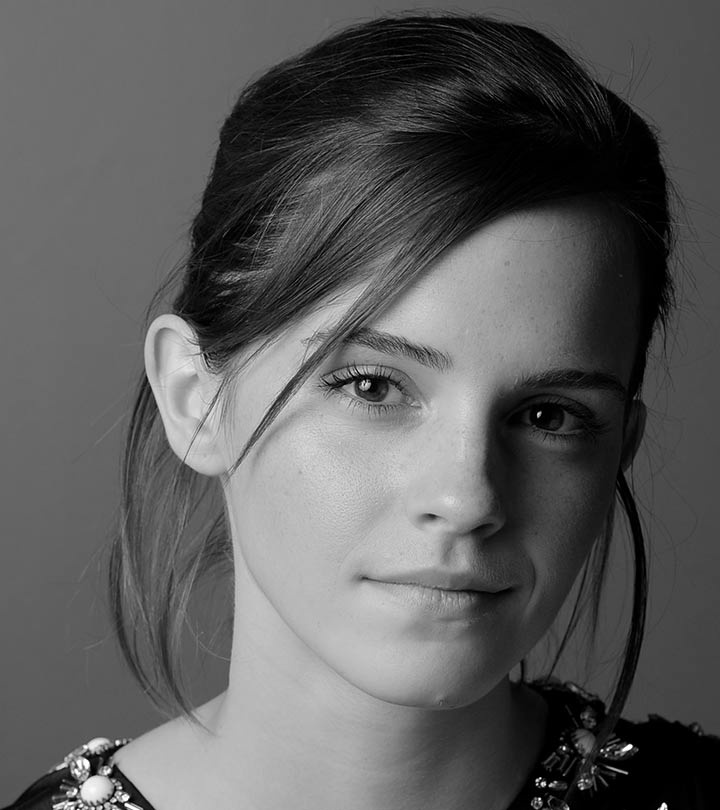
\includegraphics[width=\textwidth]{resources/emma_original.jpg}
        \caption{Original Image}
    \end{subfigure}
    \hfill
    \begin{subfigure}{0.3\textwidth}
        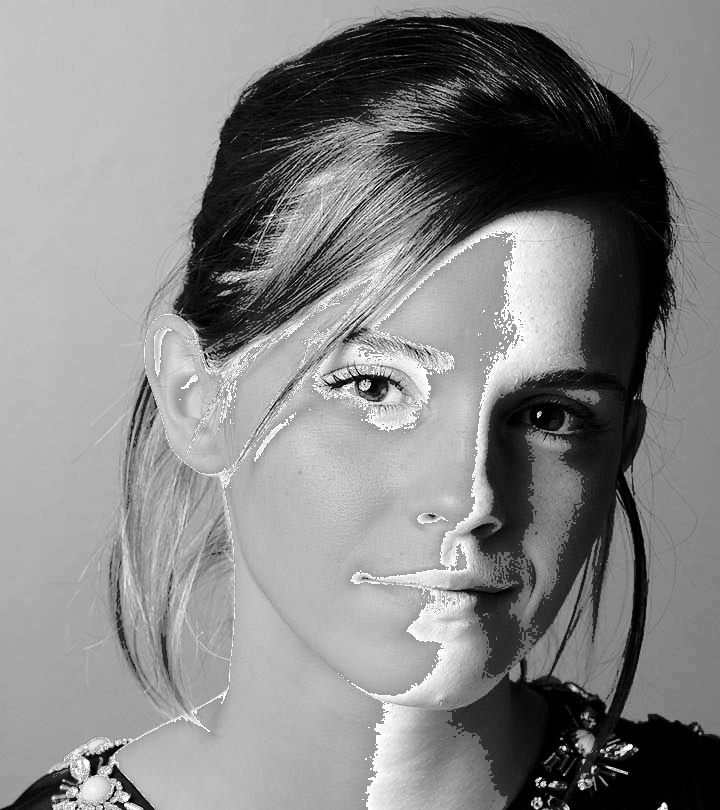
\includegraphics[width=\textwidth]{resources/emma_transformed.jpg}
        \caption{Transformed Image}
    \end{subfigure}
    \hfill
    \begin{subfigure}{0.3\textwidth}
        The transformation creates jump discontinuities that result in high contrast regions. Mid-intensity pixels are enhanced while preserving the extreme intensity values. This leads to improved visibility of features in the mid-range while maintaining the overall structure of the image.

        
    \end{subfigure}
    \caption{Intensity transformation results}
\end{figure}


% \subsection{Discussion}
% Analysis of the transformation effects and visual changes observed.
\section*{Question 2: Brain Image Enhancement}
% A histogram of the image is used to identify the intensity regions for the white matter and grey matter.

% \begin{figure}[H]
%     \centering
%     \begin{subfigure}{0.48\textwidth}
%         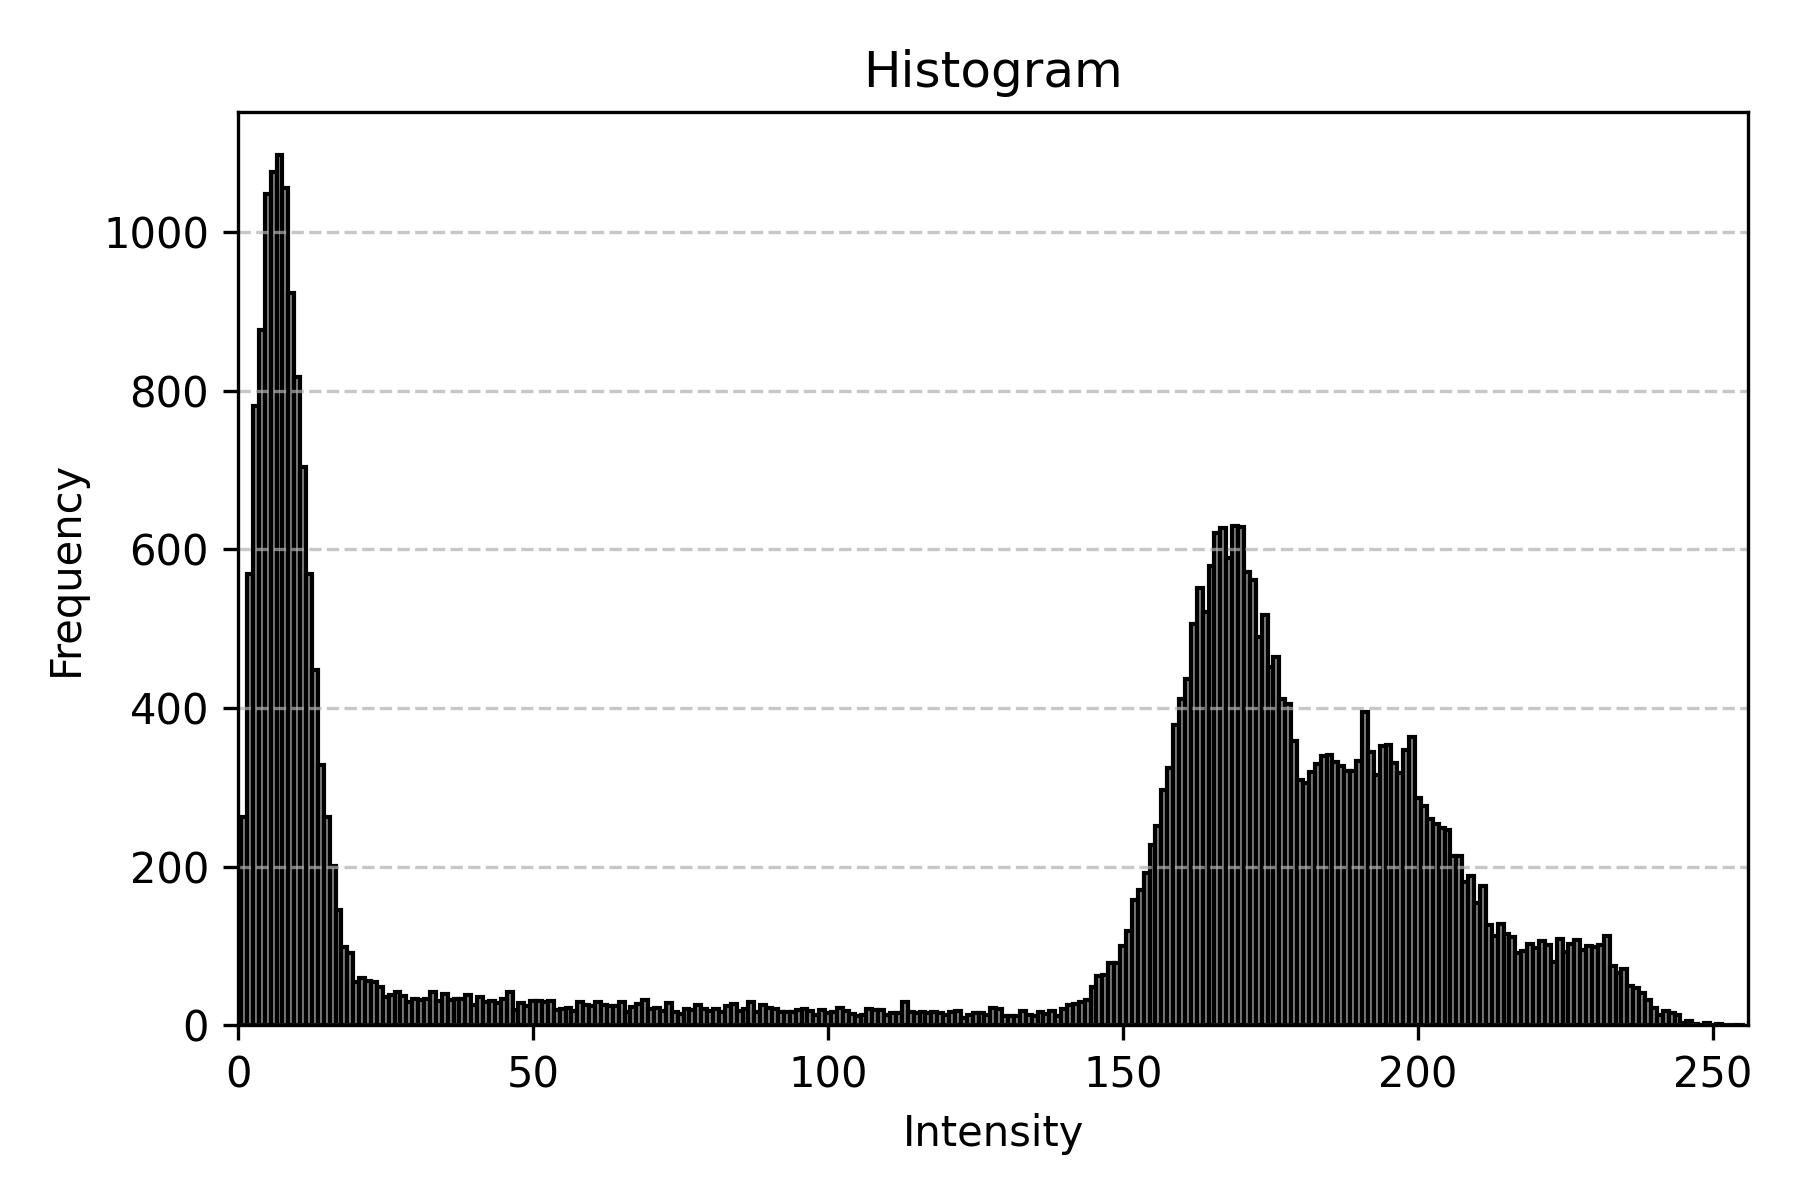
\includegraphics[width=\textwidth]{resources/Brain_hist.jpeg}
%     \end{subfigure}
%     \hfill
%     \begin{subfigure}{0.48\textwidth}
%         \begin{lstlisting}[style=pythonstyle]
% hist = cv.calcHist([img_brain], [0], None, [256], [0, 256])
%         \end{lstlisting}
%         Following intensity transformations are applied to the selected region from the histogram to enhance white matter and Grey matter regions of the brain. 
%         \vspace{3em}
%     \end{subfigure}
% \end{figure}

        \begin{lstlisting}[style=pythonstyle]
# White Matter Enhancement transformation
c = np.array([(140, 0), (180, 180)])
t1 = np.zeros(c[0, 0] + 1).astype('uint8')
t2 = np.linspace(c[0, 0] + 1, c[1, 1], c[1, 0] - c[0, 0]).astype('uint8')
t3 = np.zeros(256 - len(t1) - len(t2)).astype('uint8')
intensity_transform_white_matter_lut = np.concatenate((t1, t2, t3), axis=0).astype('uint8')
img_brain_white_matter = cv.LUT(img_brain, intensity_transform_white_matter_lut)
        \end{lstlisting}
\newpage
        \begin{lstlisting}[style=pythonstyle]
# Grey Matter Enhancement transformation
c = np.array([(180, 0), (210, 210)])
t1 = np.zeros(c[0, 0] + 1).astype('uint8')
t2 = np.linspace(c[0, 0] + 1, c[1, 1], c[1, 0] - c[0, 0]).astype('uint8')
t3 = np.zeros(256 - len(t1) - len(t2)).astype('uint8')
intensity_transform_grey_matter_lut = np.concatenate((t1, t2, t3)).astype('uint8')
img_brain_grey_matter = cv.LUT(img_brain, intensity_transform_grey_matter_lut)
        \end{lstlisting}


\begin{figure}[H]
    \centering
    \begin{subfigure}{0.2\textwidth}
        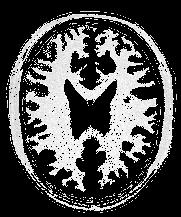
\includegraphics[width=\textwidth]{resources/whitematter_transformed_image.jpg}
        \caption{White Matter Enhanced}
    \end{subfigure}
    \hfill
    \begin{subfigure}{0.26\textwidth}
        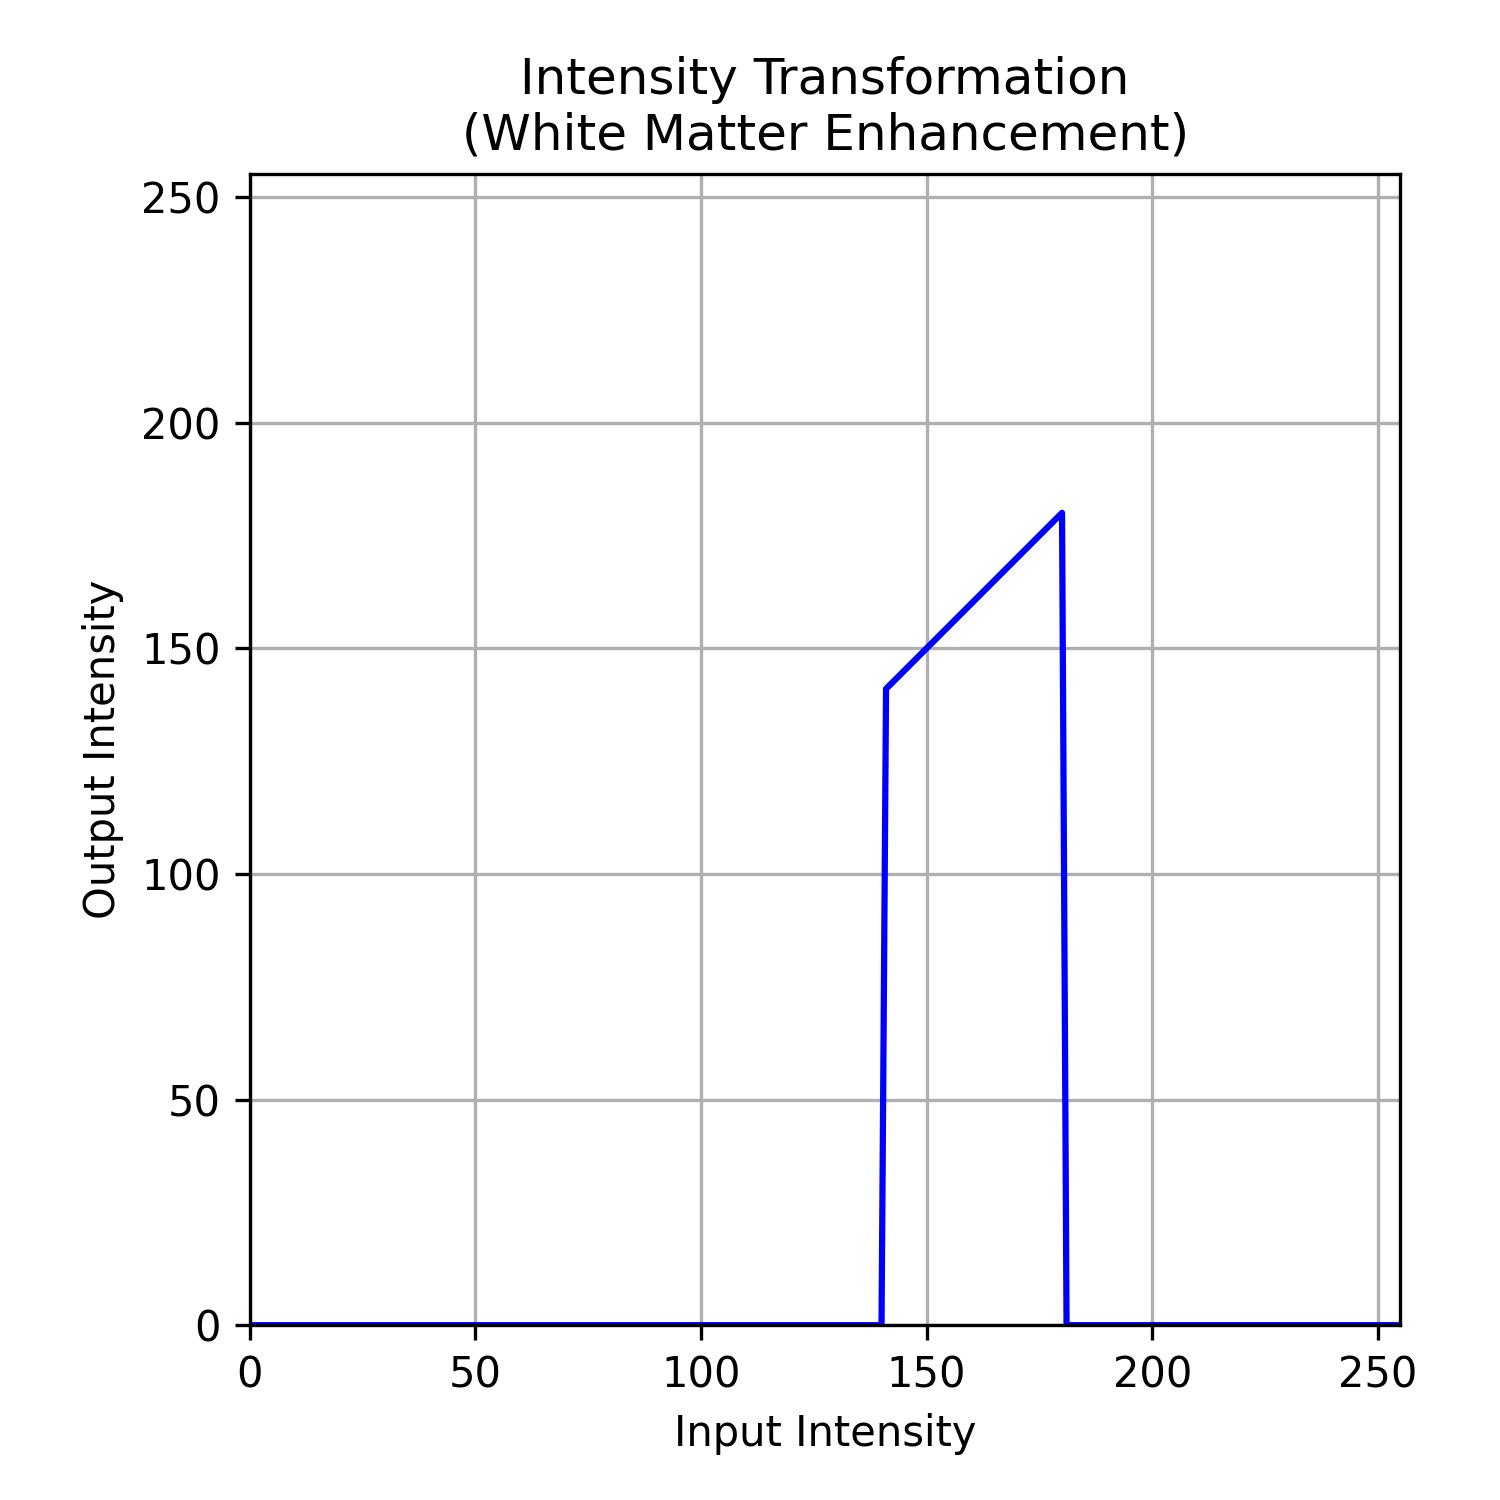
\includegraphics[width=\textwidth]{resources/Whitematter_transformation_curve.jpg}
        \caption{White Matter Plot}
    \end{subfigure}
    \hfill
    \begin{subfigure}{0.2\textwidth}
        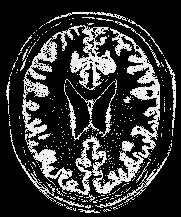
\includegraphics[width=\textwidth]{resources/transformed_gray_matter.jpg}
        \caption{Gray Matter Enhanced}
    \end{subfigure}
    \hfill
    \begin{subfigure}{0.26\textwidth}
        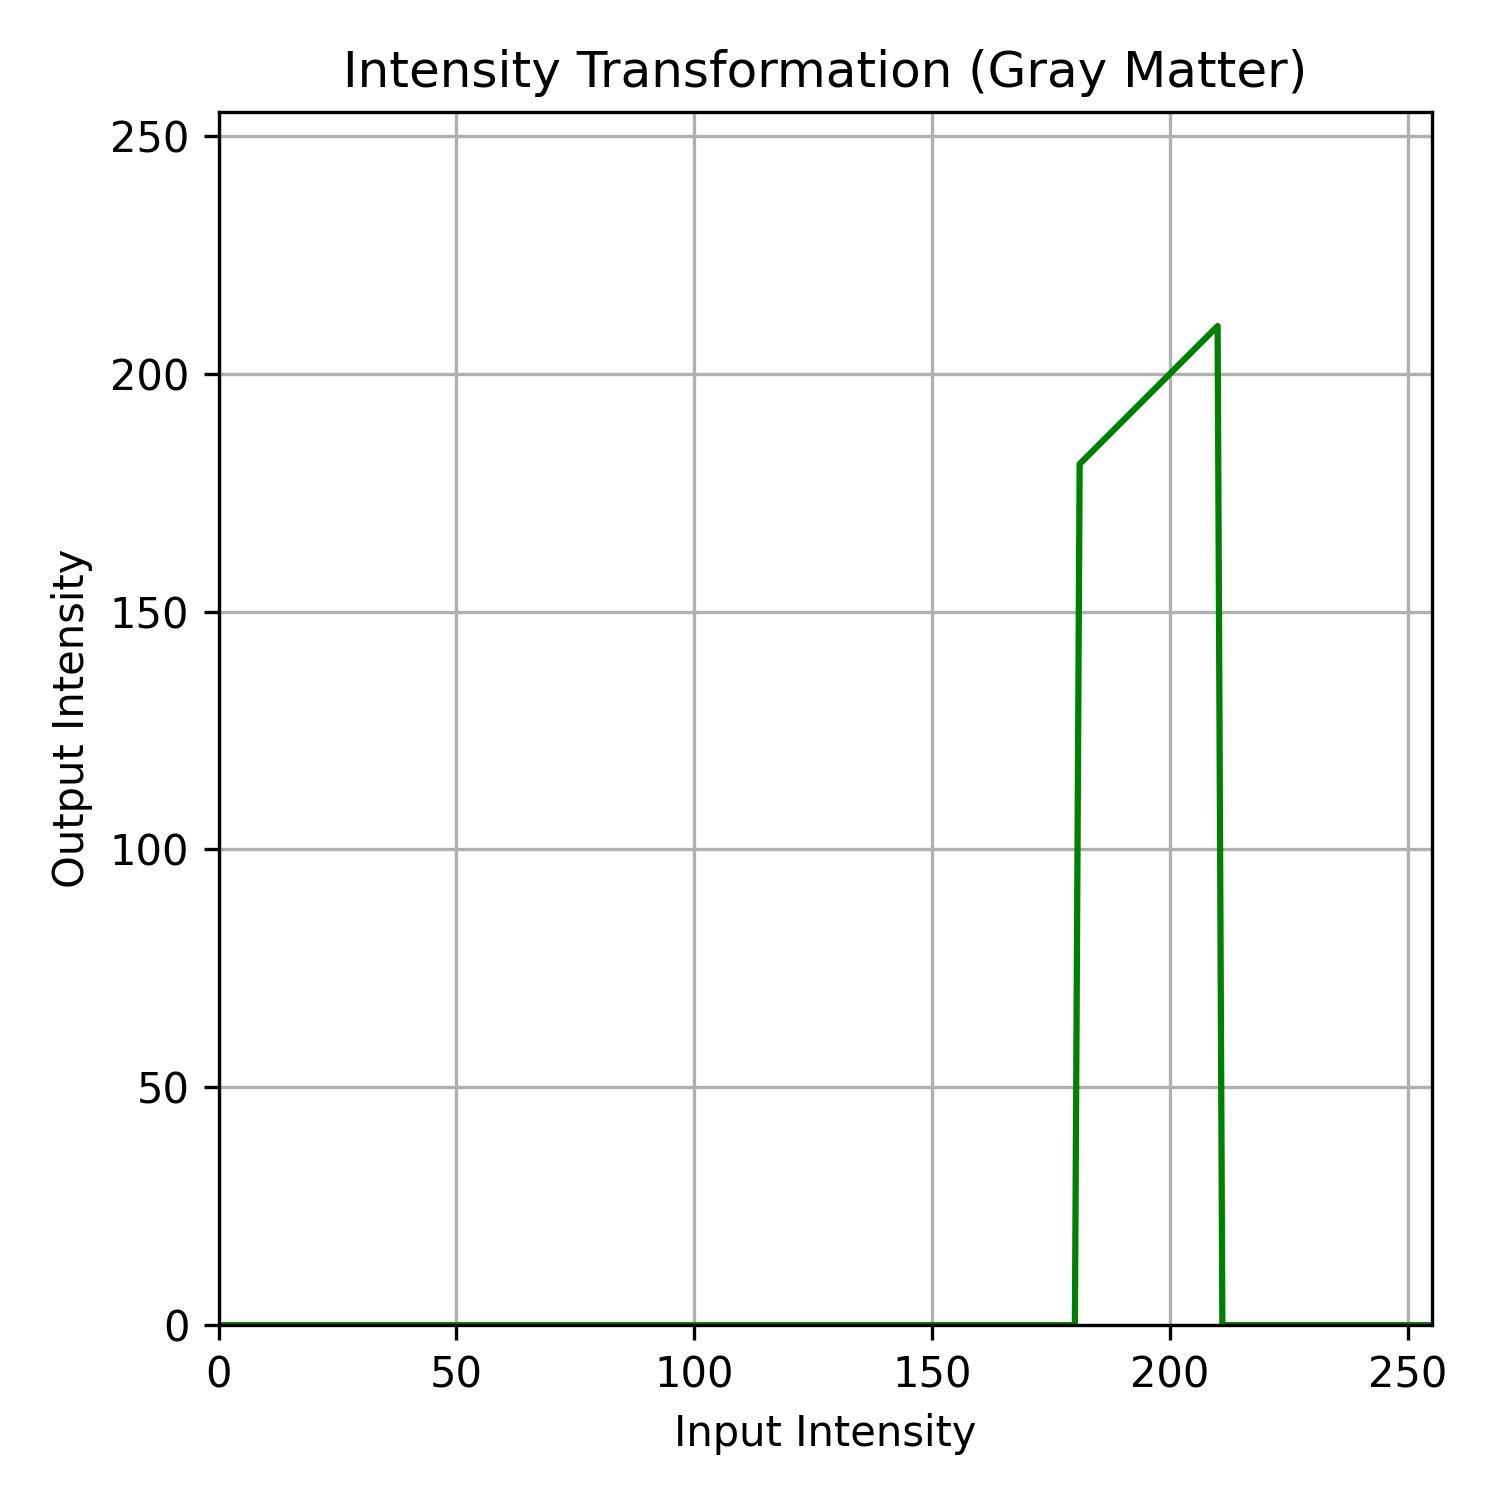
\includegraphics[width=\textwidth]{resources/transformation_curve_gray_matter.jpg}
        \caption{Gray Matter Plot}
    \end{subfigure}
    \caption{White and Gray matter enhancement results and transformation curves}
\end{figure}
The intensity transformations offer smooth contrast enhancement within specific intensity ranges, based on the color values of white and gray matter, effectively enhancing the visibility of these tissues.

\section*{Question 3: Gamma Correction}
\subsubsection*{L*a*b* Color Space Conversion}
\begin{lstlisting}[style=pythonstyle]
img_lab = cv.cvtColor(img_bgr, cv.COLOR_BGR2Lab)
L, a, b = cv.split(img_lab)
\end{lstlisting}
\subsubsection*{Applying $\gamma$ value correction}
\begin{lstlisting}[style=pythonstyle]
L_norm = L.astype(np.float32) / 255.0  
# Apply gamma correction
gamma = 0.5  # <1 brightens, >1 darkens
L_gamma = np.power(L_norm, gamma)
L_new = np.clip(L_gamma * 255.0, 0, 255).astype(np.uint8)
# Merge and convert back to BGR
img_lab_new = cv.merge((L_new, a, b))
img_bgr_new = cv.cvtColor(img_lab_new, cv.COLOR_Lab2BGR)
\end{lstlisting}
% \subsubsection*{Gamma Value Selection}
$\gamma$ value is chosen as 0.5 by comparing the images by changing the values of $\gamma$, which lightens the shadows while preserving highlights, improving overall image visibility.


\begin{figure}[H]
    \centering
    \begin{subfigure}{0.42\textwidth}
        %\fbox{\rule{0pt}{1.5in}\rule{2in}{0pt}}
        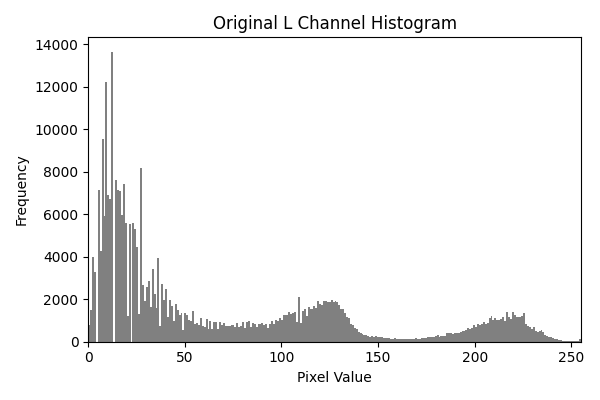
\includegraphics[width=\textwidth]{resources/gamma_original_histogram.png}
        \caption{Original L plane Histogram}
    \end{subfigure}
    \hfill
    \begin{subfigure}{0.42\textwidth}
        % \fbox{\rule{0pt}{1.5in}\rule{2in}{0pt}}
        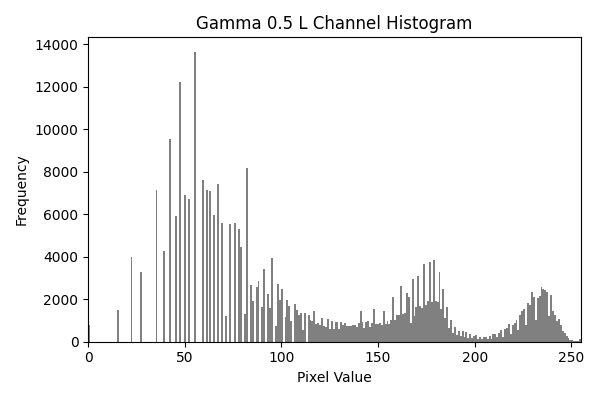
\includegraphics[width=\textwidth]{resources/gamma_0.5_histogram.png}
        \caption{Gamma Corrected L plane Histogram}
    \end{subfigure}
    %\caption{Histogram comparison before and after gamma correction}
\end{figure}

\section*{Question 4: Vibrance Enhancement}
\subsubsection*{HSV Decomposition}
\begin{lstlisting}[style=pythonstyle]
spider_hsv = cv.cvtColor(spider_img, cv.COLOR_BGR2HSV)
h, s, v = cv.split(spider_hsv)
\end{lstlisting}
\begin{figure}[H]
    \centering
    \begin{subfigure}{0.3\textwidth}
        %\fbox{\rule{0pt}{1.5in}\rule{1.5in}{0pt}}
        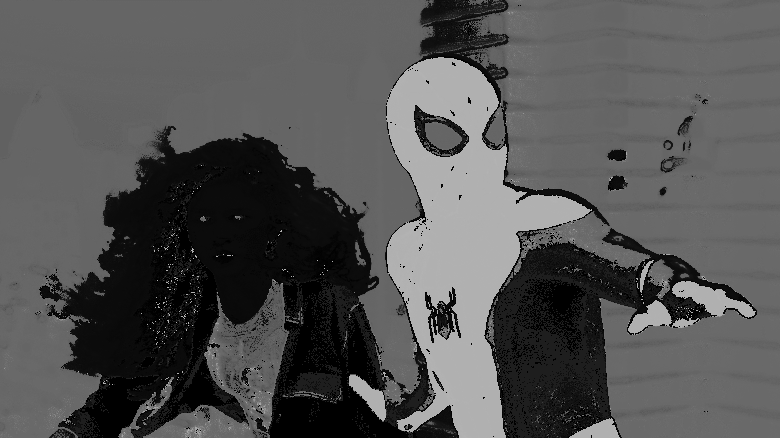
\includegraphics[width=\textwidth]{resources/spider_hue.png}
        \caption{Hue}
    \end{subfigure}
    \hfill
    \begin{subfigure}{0.3\textwidth}
        %\fbox{\rule{0pt}{1.5in}\rule{1.5in}{0pt}}
        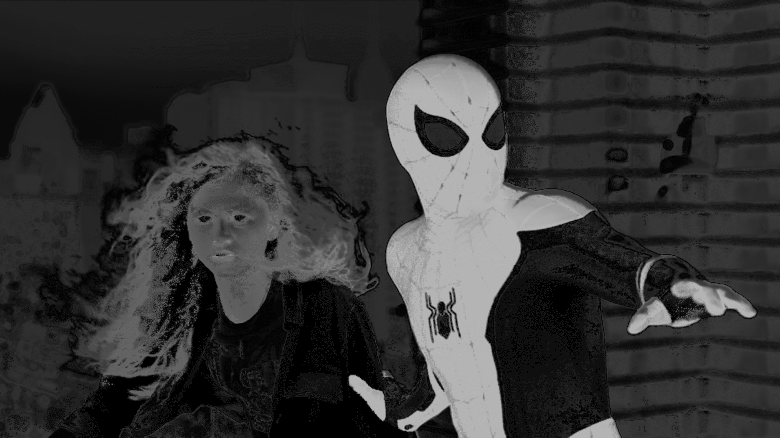
\includegraphics[width=\textwidth]{resources/spider_saturation.png}
        \caption{Saturation}
    \end{subfigure}
    \hfill
    \begin{subfigure}{0.3\textwidth}
        %\fbox{\rule{0pt}{1.5in}\rule{1.5in}{0pt}}
        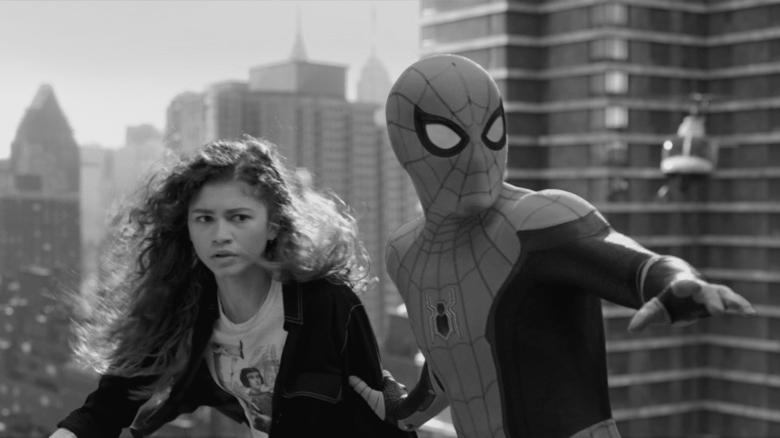
\includegraphics[width=\textwidth]{resources/spider_value.png}
        \caption{Value}
    \end{subfigure}
    \caption{HSV plane decomposition}
\end{figure}

\subsubsection*{Vibrance Transformation}

\begin{lstlisting}[style=pythonstyle]
def transformation(x: np.ndarray, a: float, sigma: int=70) -> np.ndarray:
    x_float = x.astype(np.float64) # To stop overflow
    exponent = -1 * (x_float - 128)**2 / (2 * sigma**2)
    fx = x_float + a * 128 * np.exp(exponent)
    return np.clip(fx, 0, 255).astype(np.uint8)
\end{lstlisting}

\subsubsection*{Applying the transformation}
\begin{lstlisting}[style=pythonstyle]
a_val = 0.7  
sigma_val = 70
s_transformed = transformation(s, a=a_val, sigma=sigma_val)
spider_hsv_transformed = cv.merge([h, s_transformed, v])
spider_transformed_bgr = cv.cvtColor(spider_hsv_transformed, cv.COLOR_HSV2BGR)
\end{lstlisting}

A value of $a = 0.7$ was chosen to provide a balanced enhancement of image vibrance without introducing oversaturation or unnatural colors. At this level, colorful regions are noticeably intensified, improving visual appeal, while grayscale and low-saturation regions remain largely unaffected. This ensures that the transformation selectively enhances vivid areas without distorting the overall color balance, making it suitable for natural-looking vibrance enhancement.

\subsubsection*{Results Comparison}
%Show original, enhanced, and transformation curve.
\begin{figure}[H]
    \centering
    \begin{subfigure}{0.33\textwidth}
        %\fbox{\rule{0pt}{1.5in}\rule{1.5in}{0pt}}
        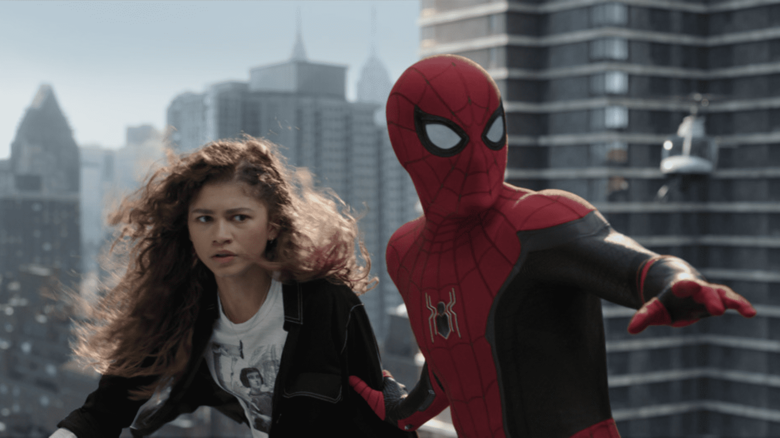
\includegraphics[width=\textwidth]{resources/spider.png}
        \caption{Original Image}
    \end{subfigure}
    \hfill
    \begin{subfigure}{0.33\textwidth}
        %\fbox{\rule{0pt}{1.5in}\rule{1.5in}{0pt}}
        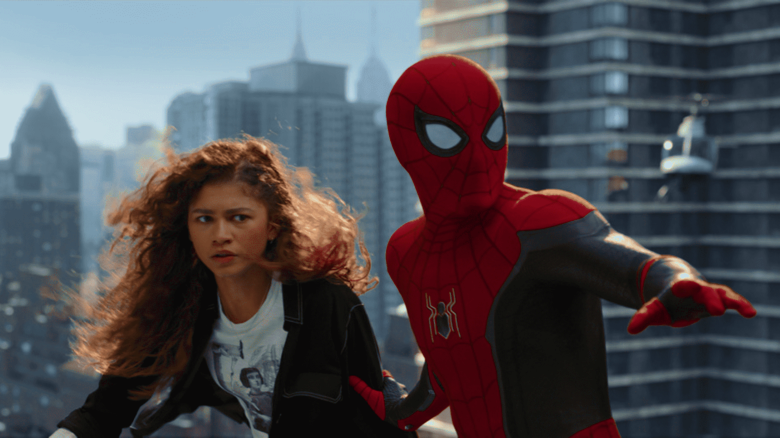
\includegraphics[width=\textwidth]{resources/spider_transformed.png}
        \caption{Vibrance-enhanced image}
    \end{subfigure}
    \hfill
    \begin{subfigure}{0.3\textwidth}
        %\fbox{\rule{0pt}{1.5in}\rule{1.5in}{0pt}}
        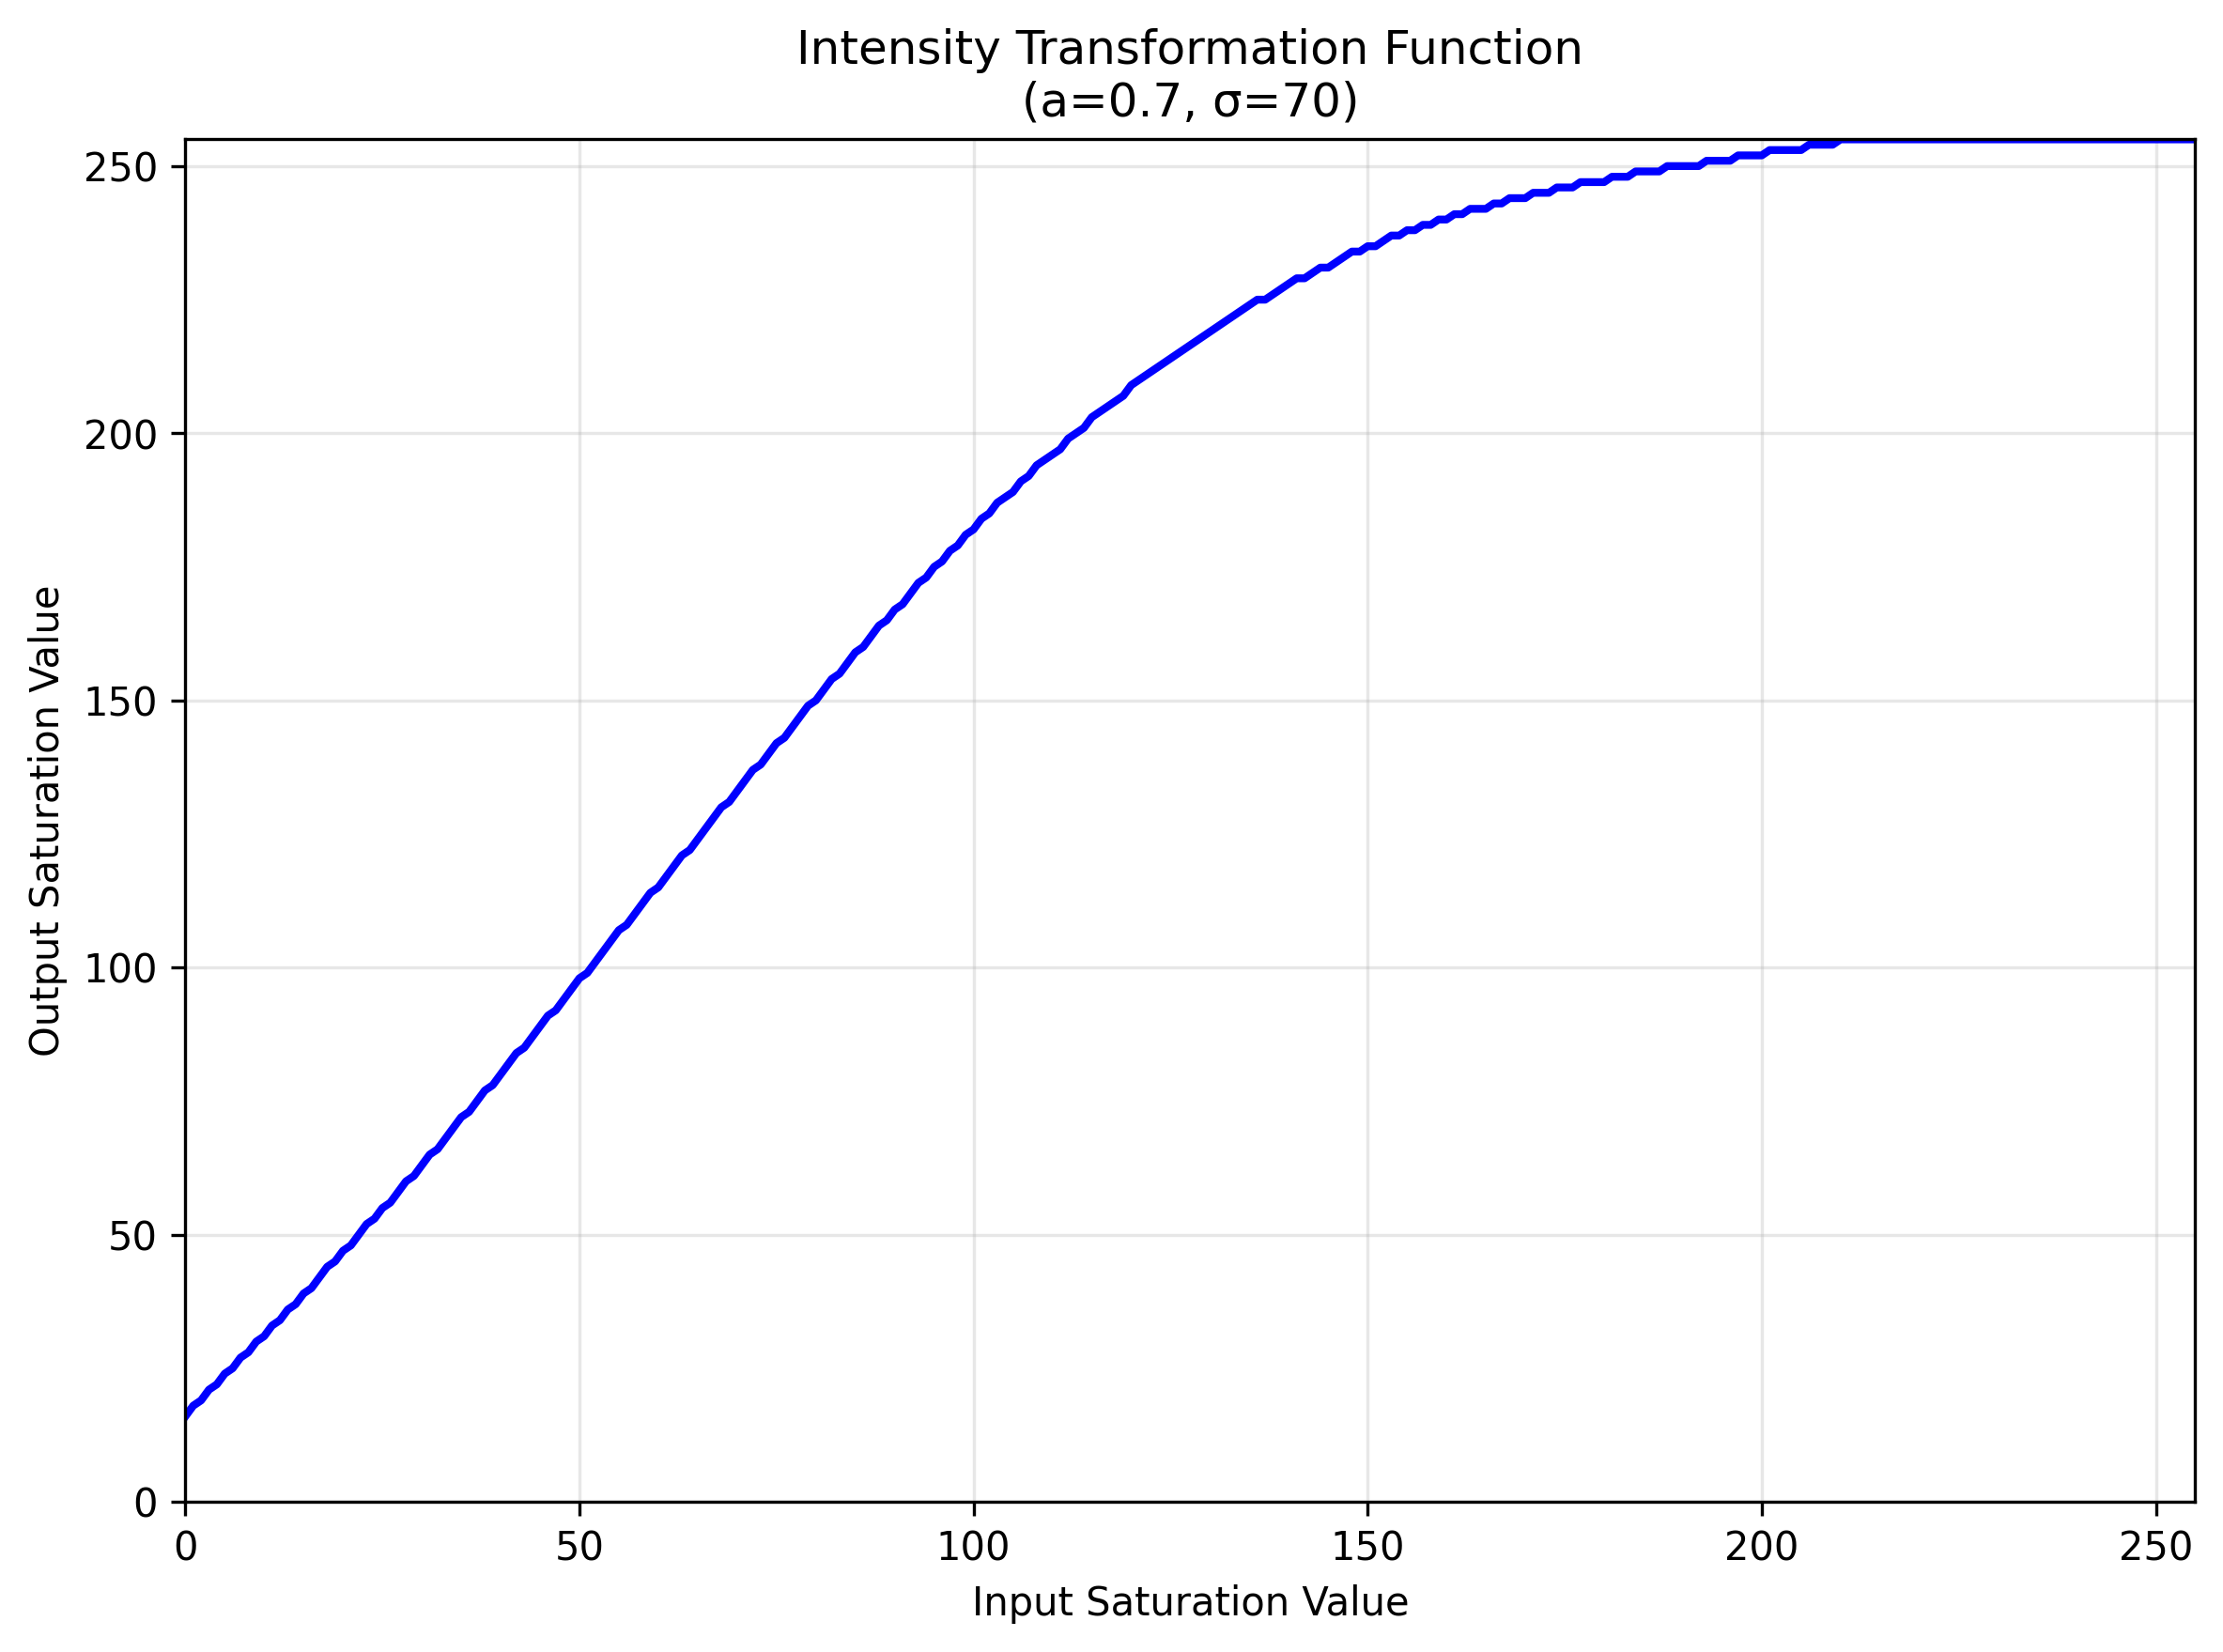
\includegraphics[width=\textwidth]{resources/spider_transformation_graph.png}
        \caption{Intensity Transformation}
    \end{subfigure}
    \caption{HSV plane decomposition}
\end{figure}
\newpage
\section*{Question 5: Histogram Equalization}

\begin{lstlisting}[style=pythonstyle]
def calculate_histogram(image: np.ndarray, height: int, width) -> np.ndarray:
    # Calculate histogram
    hist = np.zeros(256)
    for i in range(height):
        for j in range(width):
            hist[image[i, j]] += 1
    return hist

def calculate_cdf(image: np.ndarray, height, width):
    # Calculate cumulative distribution function (CDF)
    total_pixels = height * width
    hist = calculate_histogram(image, height, width)
    cdf = np.zeros(256)
    cdf[0] = hist[0]
    for i in range(1, 256):
        cdf[i] = cdf[i-1] + hist[i]
    # Normalize CDF
    cdf_normalized = cdf / total_pixels
    return cdf_normalized, hist

def histogram_equalization(image: np.ndarray) -> np.ndarray:
    height, width = image.shape
    total_pixels = height * width
    original_cdf, original_histogram = calculate_cdf(image, height, width)
    # Apply transformation
    equalized_image = np.zeros_like(image)
    for i in range(height):
        for j in range(width):
            equalized_image[i, j] = (255 * original_cdf[image[i, j]]).astype(np.uint8)
    return equalized_image


img = cv.imread("./a1images/shells.tif", cv.IMREAD_GRAYSCALE)
equalized_img = histogram_equalization(img, debug=True)
\end{lstlisting}


\subsubsection*{Results and Analysis}
\begin{figure}[H]
    \centering
    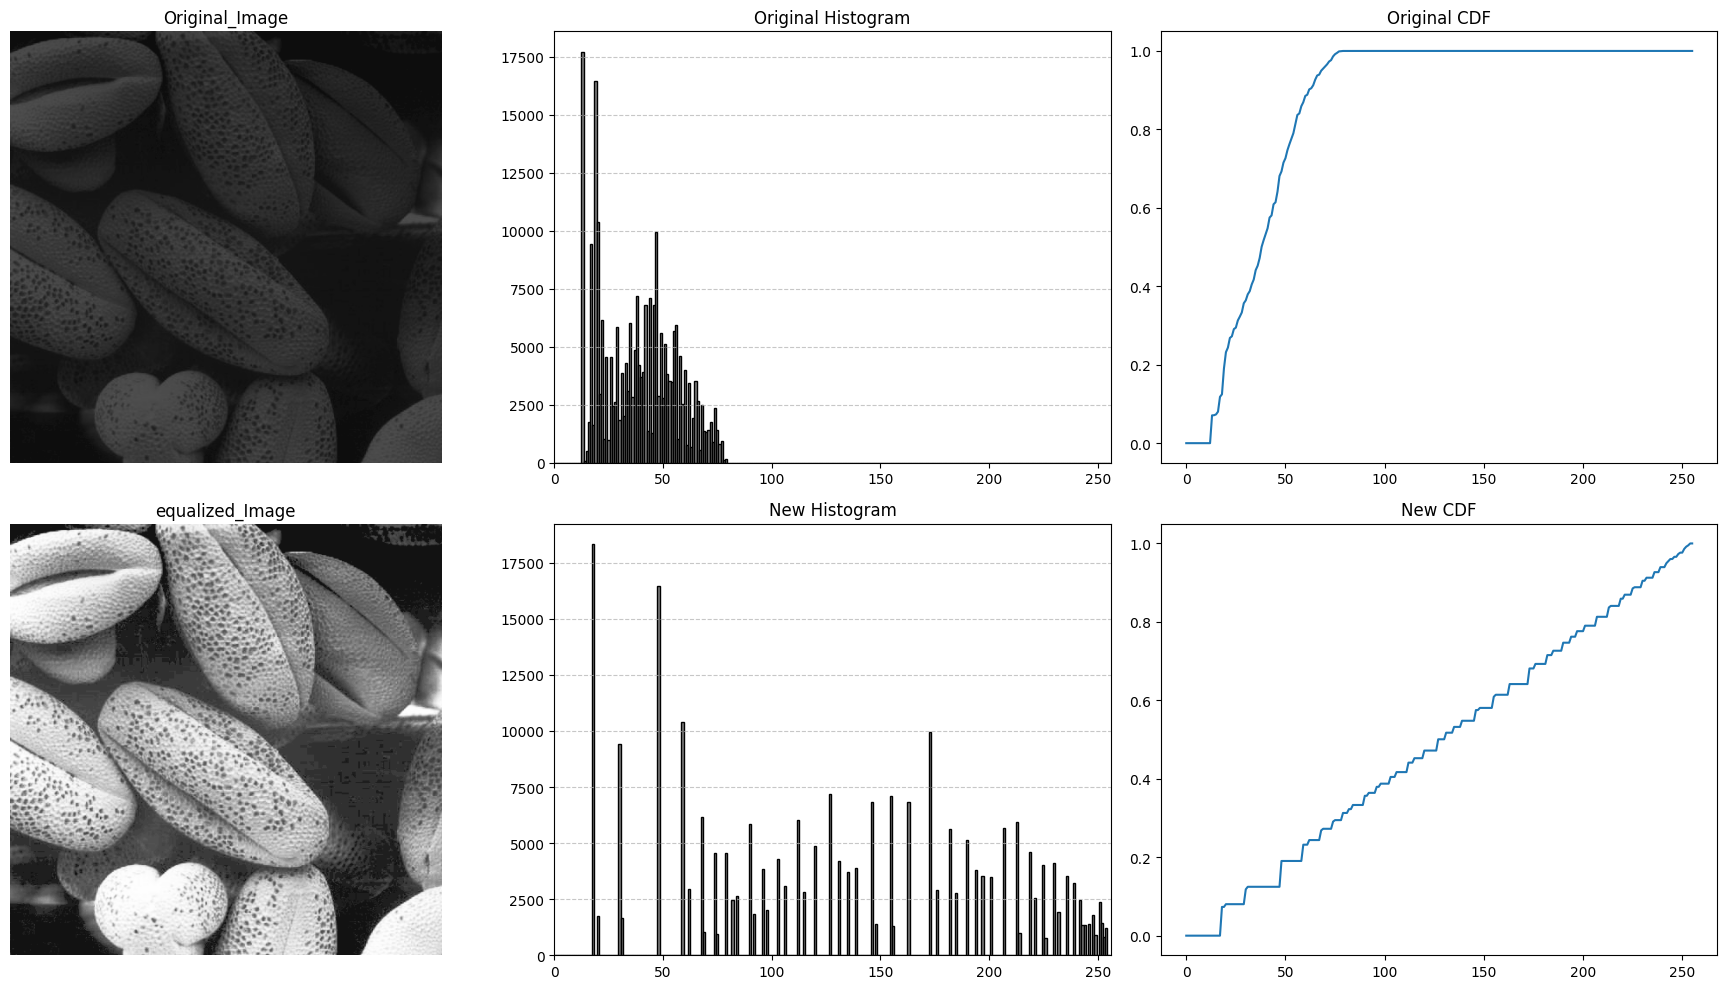
\includegraphics[width=1\linewidth]{resources/custom_his_eq.png}
    %\caption{Caption}
    \label{fig:placeholder}
\end{figure}
\newpage
\section*{Question 6: Foreground Histogram Equalization}
\subsubsection*{HSV Analysis and Masking}
The Saturation channel is selected as it provides clear separation of the foreground based on color intensity, effectively isolating the subject.
\begin{figure}[H]
    \centering
    \begin{subfigure}{0.3\textwidth}
        %\fbox{\rule{0pt}{1.5in}\rule{1.5in}{0pt}}
        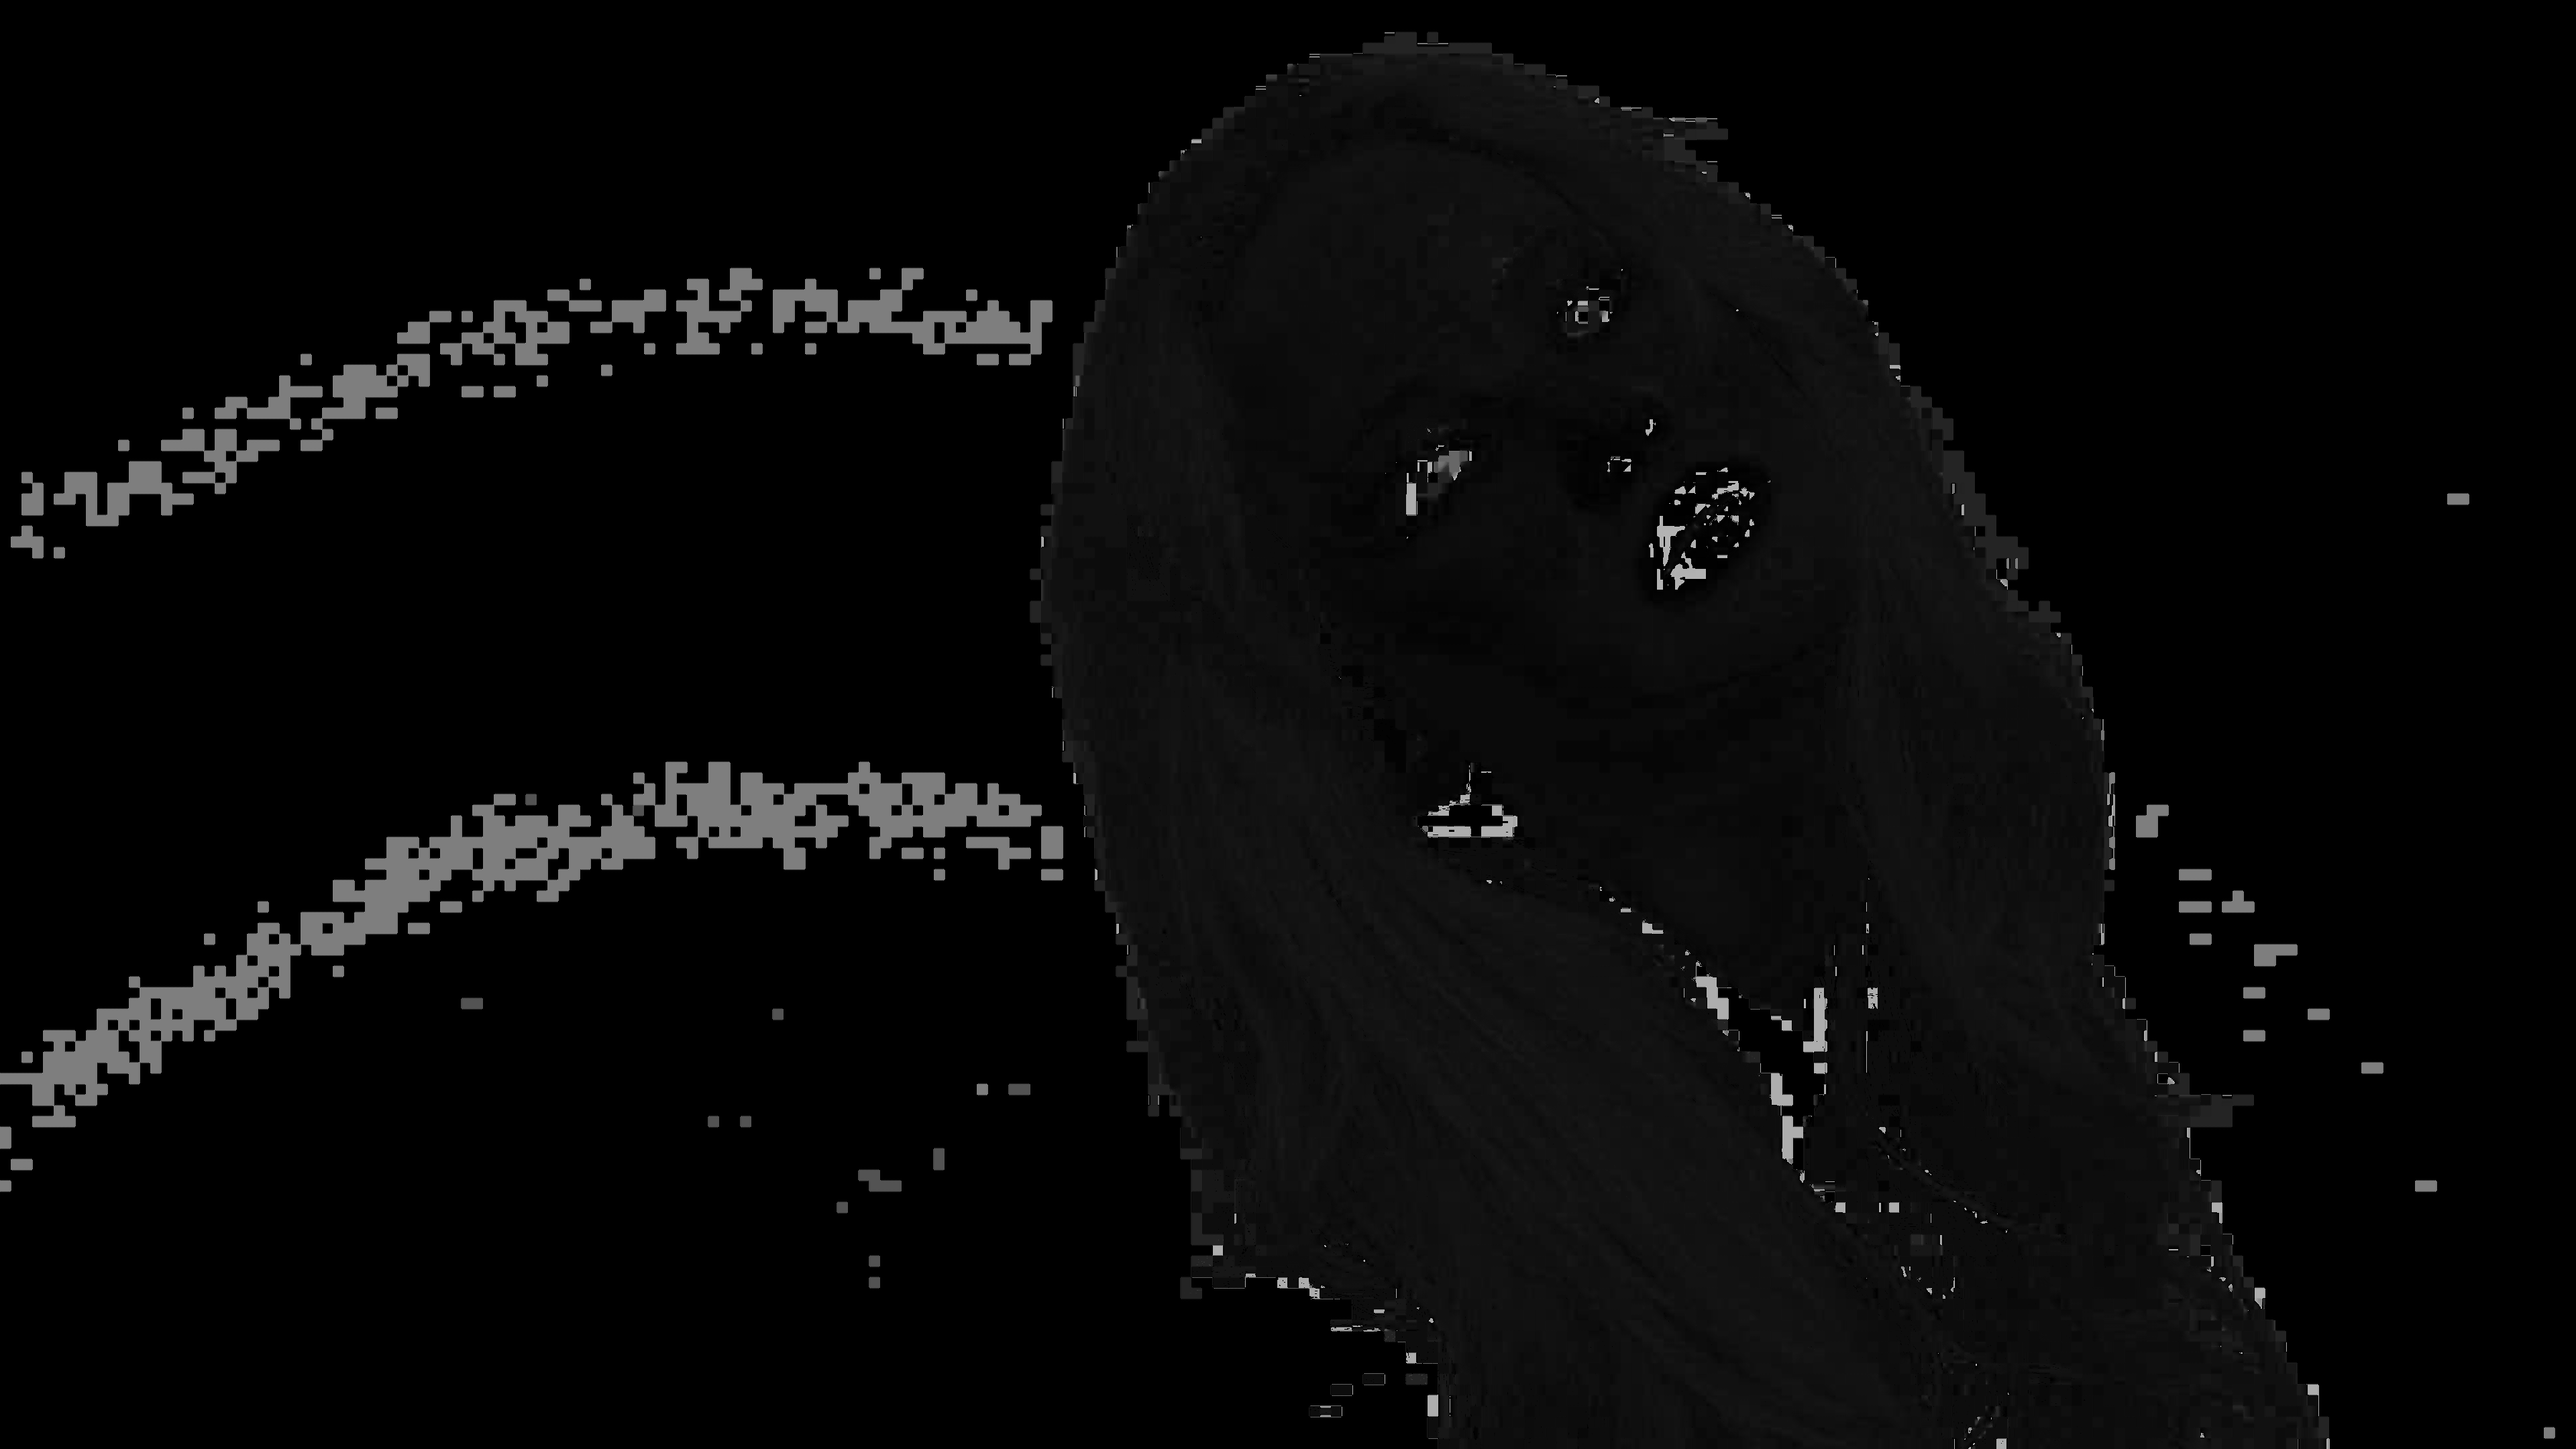
\includegraphics[width=\textwidth]{resources/jeniffer_hue.png}
        \caption{Hue}
    \end{subfigure}
    \hfill
    \begin{subfigure}{0.3\textwidth}
        %\fbox{\rule{0pt}{1.5in}\rule{1.5in}{0pt}}
        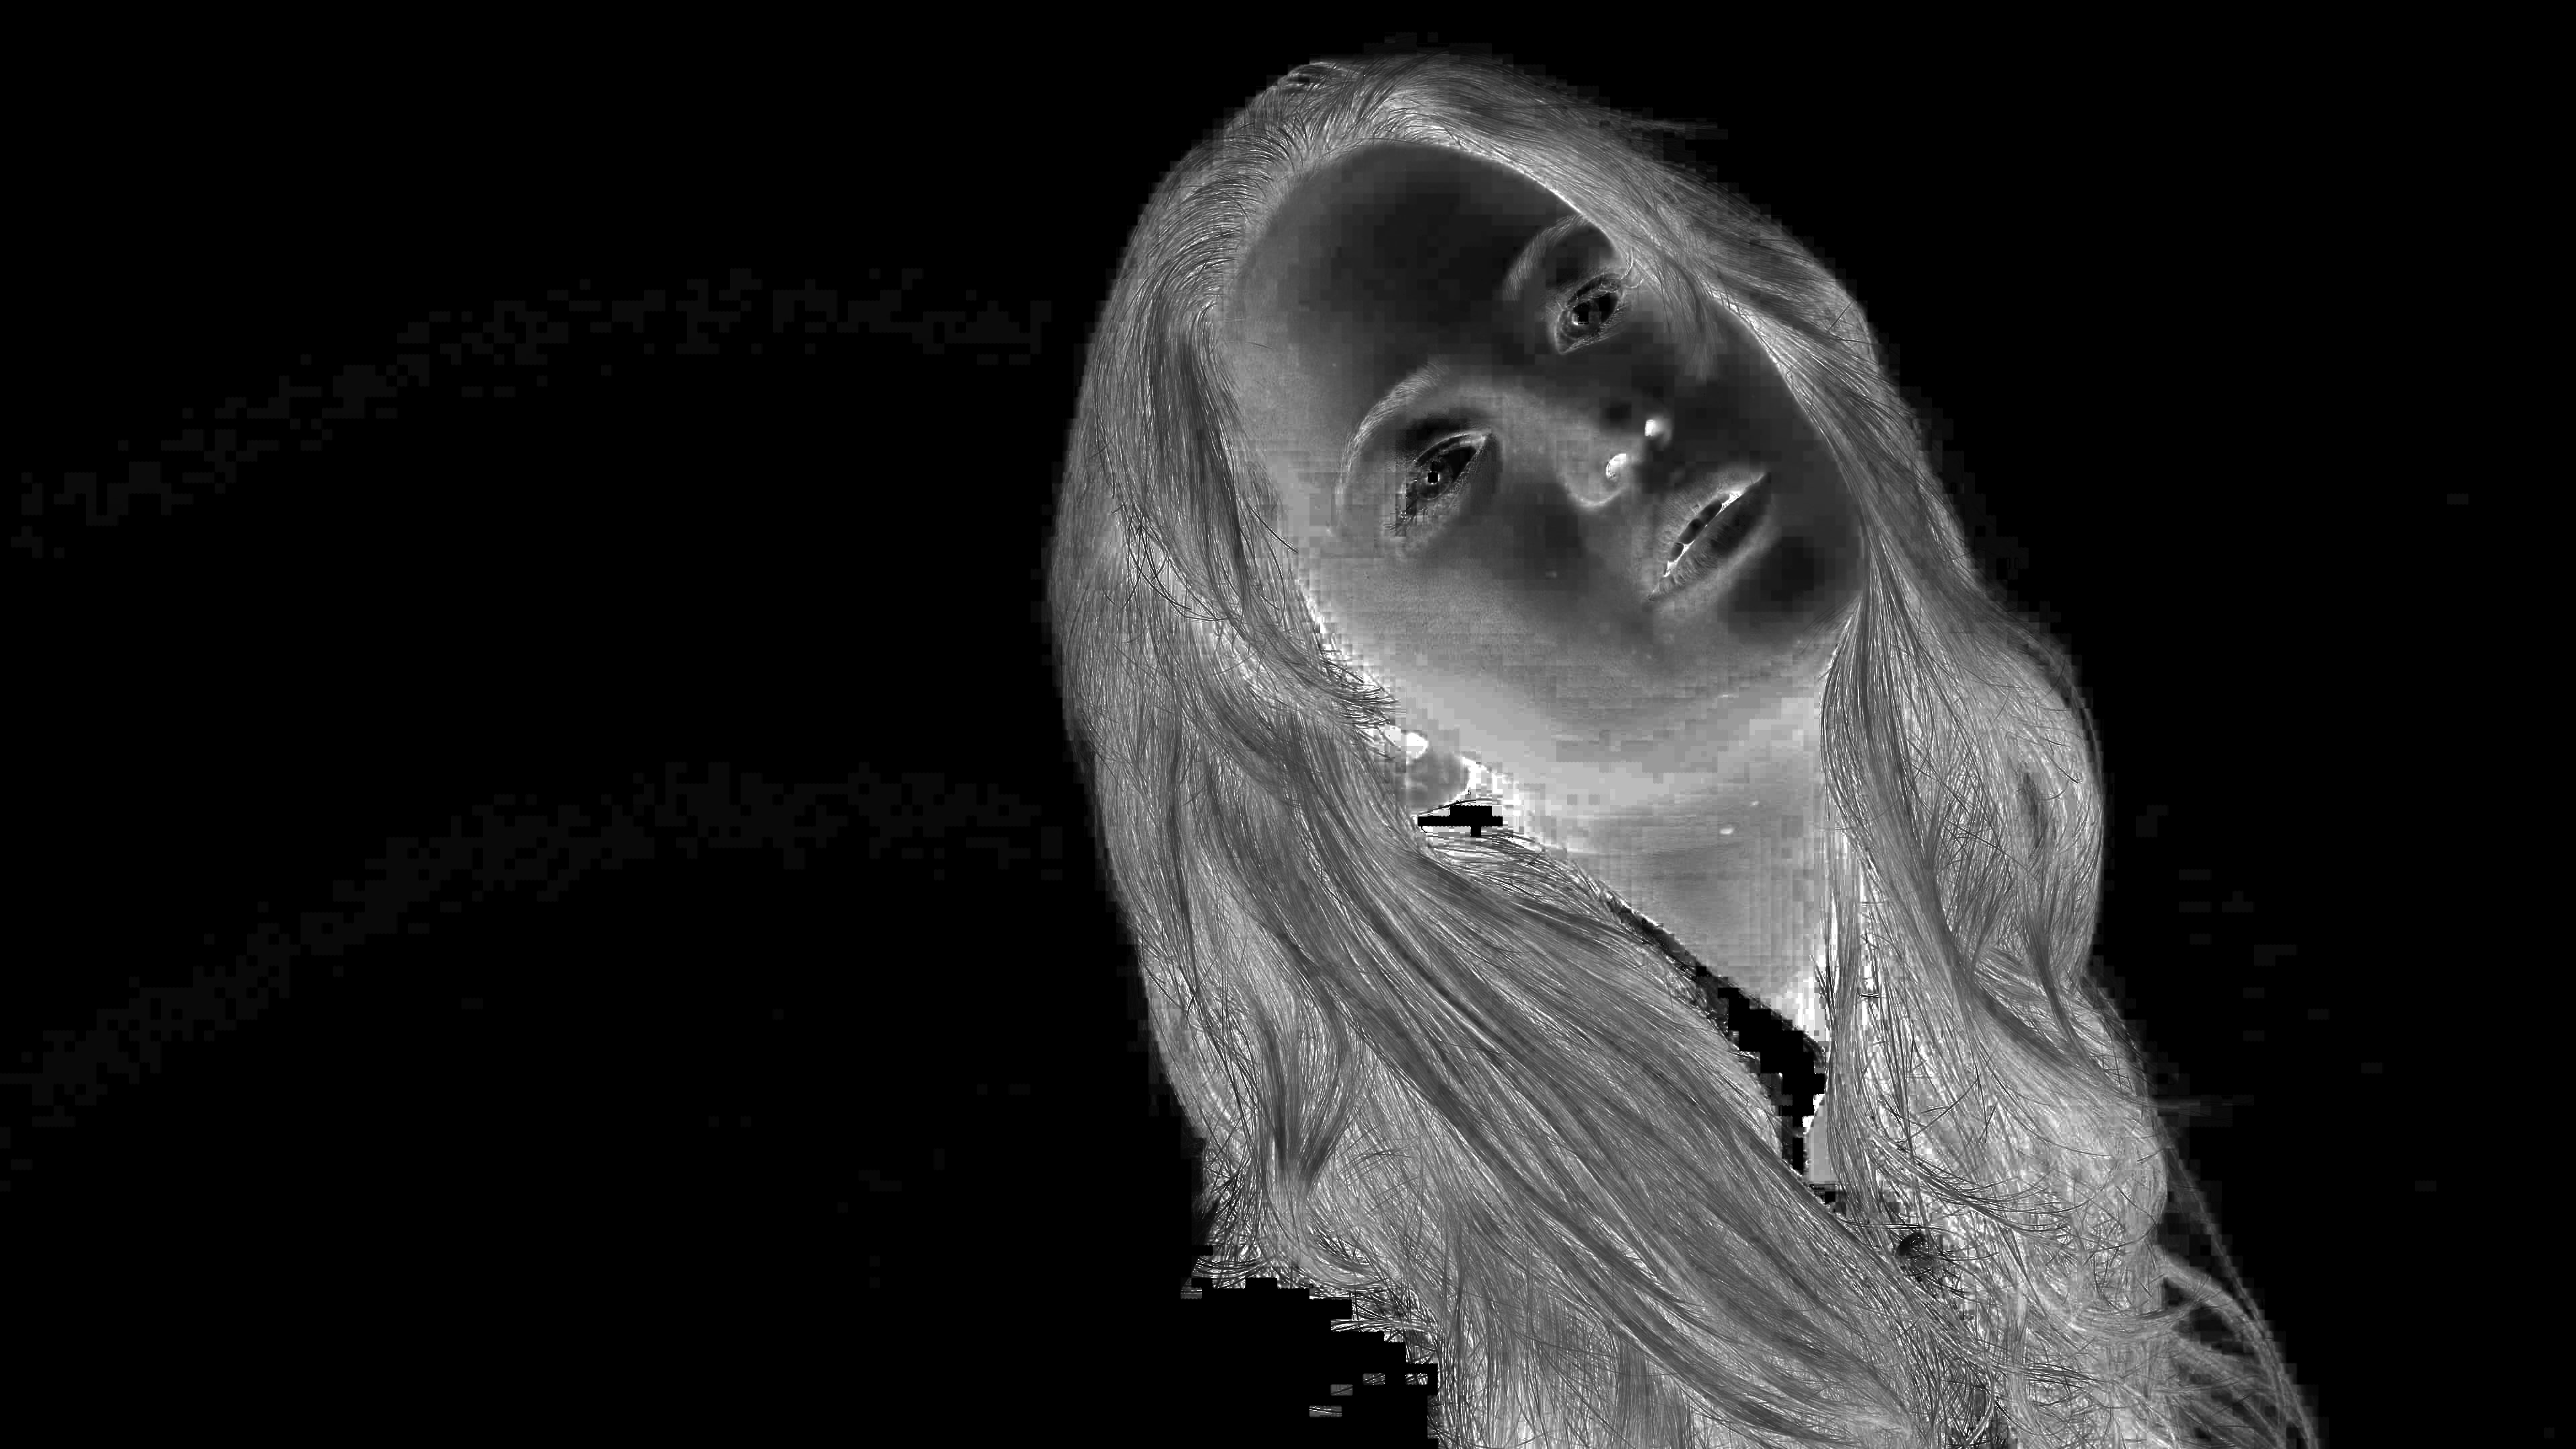
\includegraphics[width=\textwidth]{resources/jeniffer_saturation.png}
        \caption{Saturation}
    \end{subfigure}
    \hfill
    \begin{subfigure}{0.3\textwidth}
        %\fbox{\rule{0pt}{1.5in}\rule{1.5in}{0pt}}
        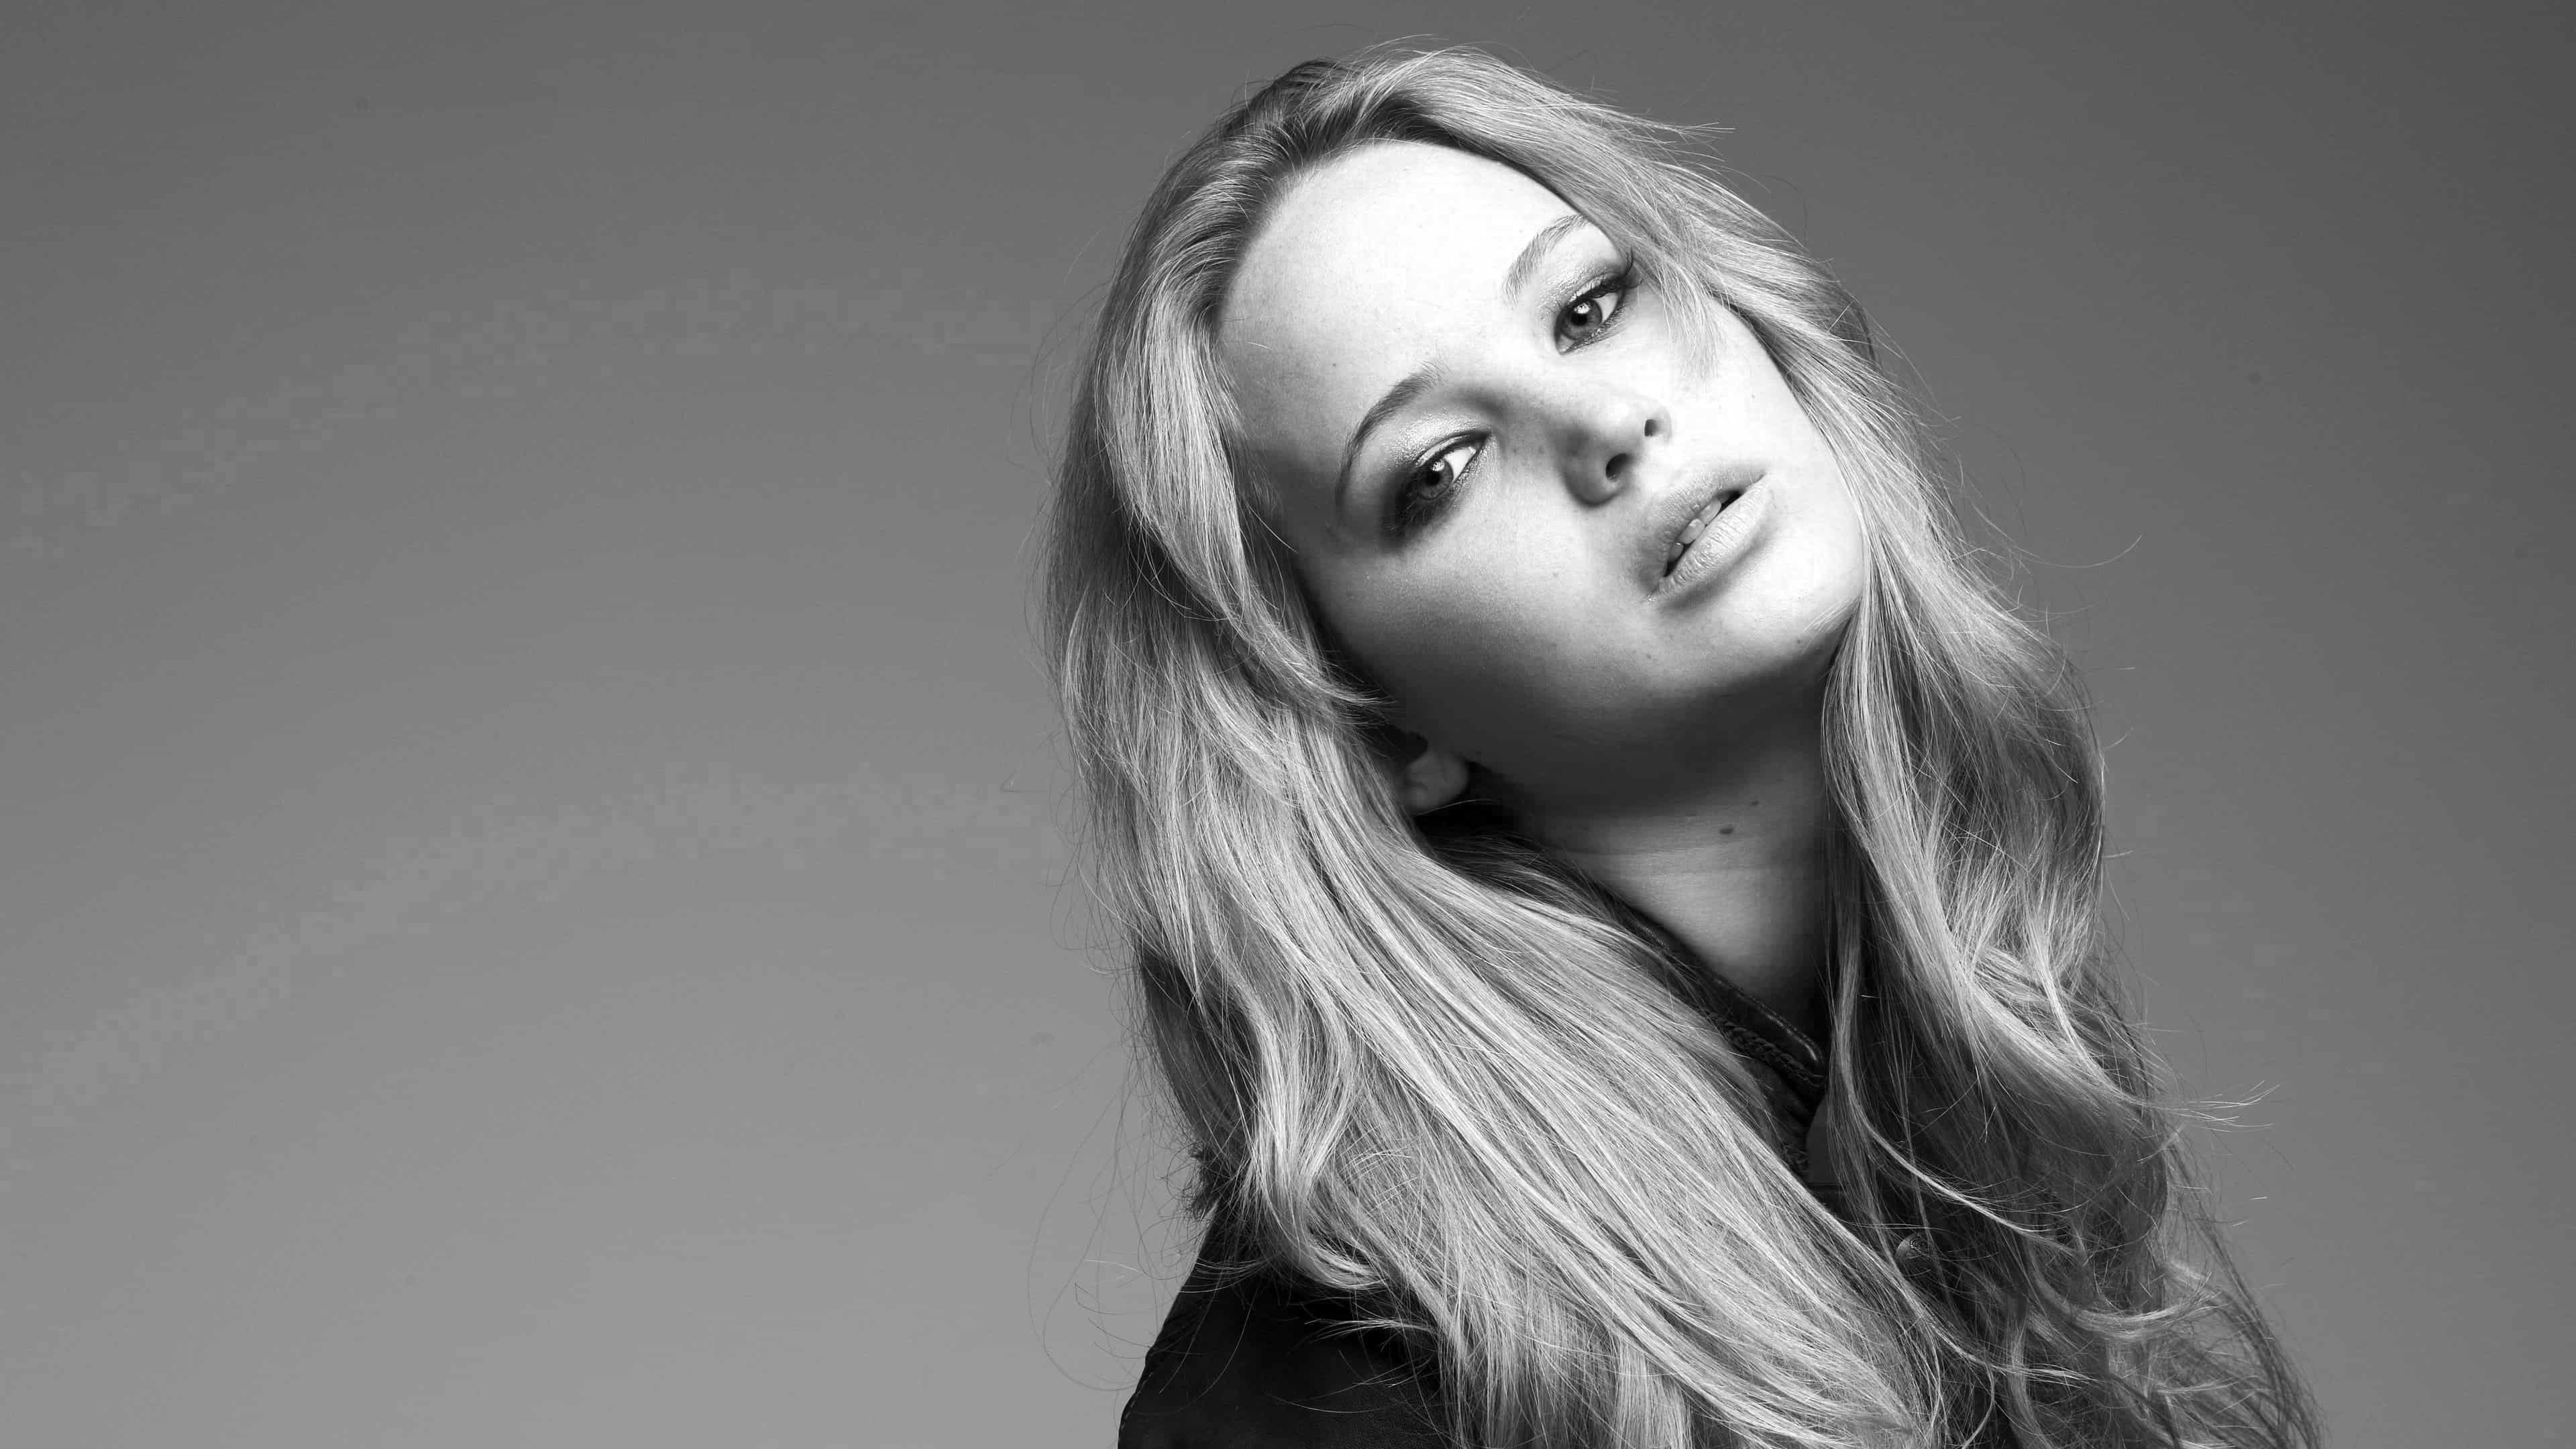
\includegraphics[width=\textwidth]{resources/jeniffer_value.png}
        \caption{Value}
    \end{subfigure}
    \caption{HSV plane decomposition}
\end{figure}

\subsubsection*{Foreground Extraction}
\begin{lstlisting}[style=pythonstyle]
threshold_value = 13  
_, mask = cv.threshold(s, threshold_value, 255, cv.THRESH_BINARY)

foreground = cv.bitwise_and(jeniffer_img, jeniffer_img, mask=mask)
 # Compute histogram of the value channel for foreground pixels only
foreground_v = cv.bitwise_and(v, v, mask=mask)
\end{lstlisting}

\begin{figure}[H]
    \centering
    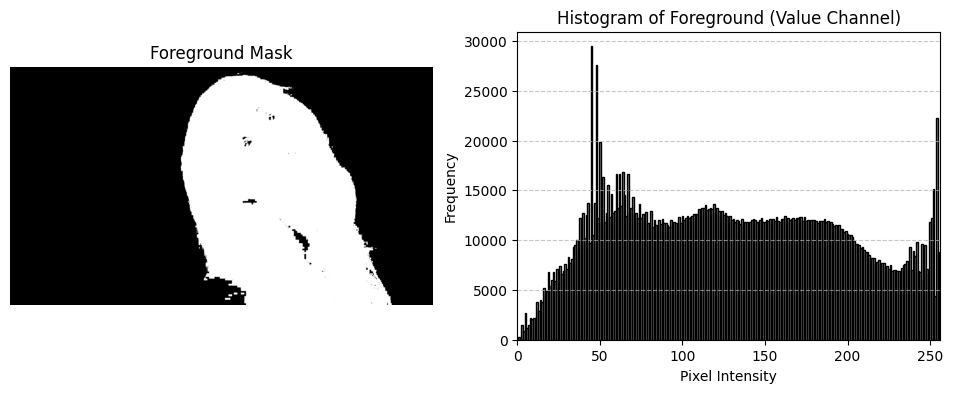
\includegraphics[width=0.8\linewidth]{resources/jeniffer_mask_hist.png}
    %\caption{Caption}
    \label{fig:placeholder}
\end{figure}

\subsubsection*{Selective Histogram Equalization}
Application of histogram equalization only to the foreground.
\begin{lstlisting}[style=pythonstyle]
cumsum = np.cumsum(hist_original)
cumsum_normalized = cumsum * 255 / cumsum[-1]   # Normalize cumulative sum

lut = np.zeros(256, dtype=np.uint8)     # Create lookup table 
for i in range(256):
    lut[i] = int(cumsum_normalized[i])
    
# Apply histogram equalization only to foreground pixels
v_equalized = v.copy()
v_equalized[mask > 0] = lut[v[mask > 0]]

hsv_equalized = cv.merge([h, s, v_equalized])
\end{lstlisting}
\newpage
\subsubsection*{Results}
Selective equalization enhances foreground details while preserving the background, resulting in improved contrast and clearer distinction of the subject.

\begin{figure}[H]
    \centering
    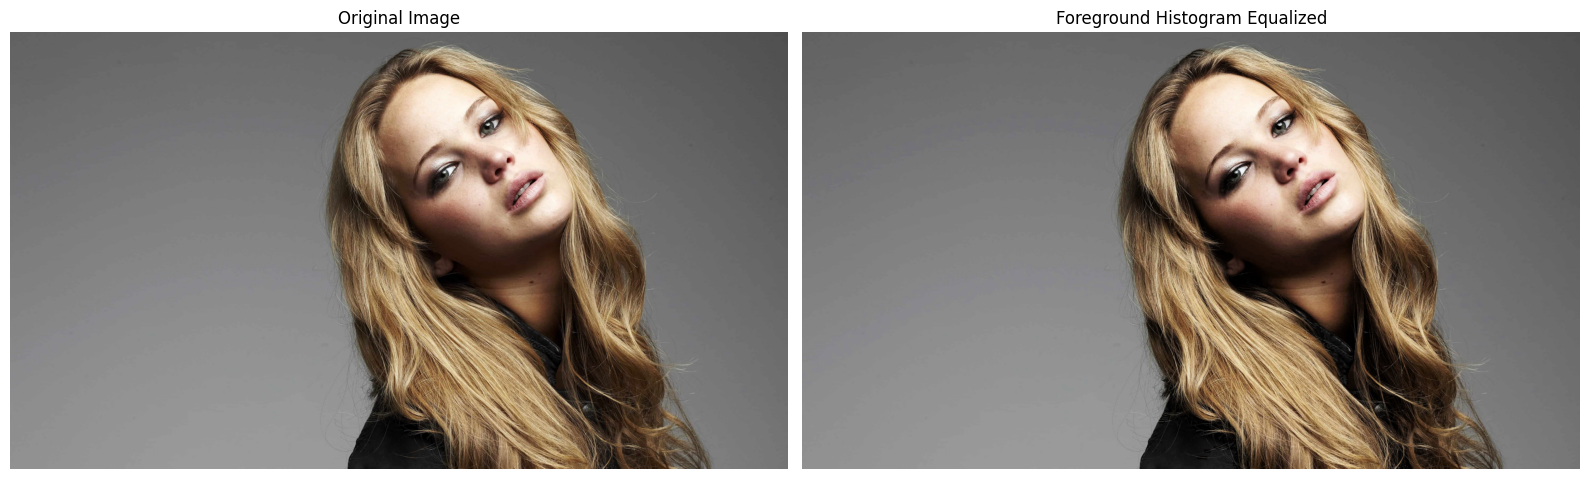
\includegraphics[width=0.95\linewidth]{resources/histogram_equalized_foreground.png}
    %\caption{Caption}
    \label{fig:placeholder}
\end{figure}

\section*{Question 7: Sobel Filtering}
\subsubsection*{Method 1: Using filter2D}
\begin{lstlisting}[style=pythonstyle]
sobel_x = np.array([[-1, -2, -1],
                    [0, 0, 0],
                    [1, 2, 1]])

sobel_y = np.array([[-1, 0, 1],
                    [-2, 0, 2],
                    [-1, 0, 1]])

einstein_sobel_x = cv.filter2D(einstein_img, cv.CV_64F, sobel_x)
einstein_sobel_y = cv.filter2D(einstein_img, cv.CV_64F, sobel_y)
\end{lstlisting}


\subsubsection*{Method 2: Custom Implementation}
\begin{lstlisting}[style=pythonstyle]
def sobel_convolution(image, kernel):
    h, w = image.shape
    kh, kw = kernel.shape
    pad_h, pad_w = kh // 2, kw // 2
    padded = np.pad(image, ((pad_h, pad_h), (pad_w, pad_w)), mode='constant')
    output = np.zeros_like(image, dtype=np.float64)
    for i in range(h):
        for j in range(w):
            region = padded[i:i+kh, j:j+kw]
            output[i, j] = np.sum(region * kernel)
    
    return output

sobel_x_manual = sobel_convolution(einstein_img, sobel_x)
sobel_y_manual = sobel_convolution(einstein_img, sobel_y)
\end{lstlisting}

\subsubsection*{Method 3: Separable Filters}
\begin{lstlisting}[style=pythonstyle]
kx = np.array([1, 0, -1], dtype=np.float32).reshape(1, 3)
ky = np.array([1, 2, 1], dtype=np.float32).reshape(3, 1)
# First filter horizontally, then vertically
temp = cv.filter2D(einstein_img, cv.CV_64F, kx)
sobel_x_sep = cv.filter2D(temp, cv.CV_64F, ky)

\end{lstlisting}

\begin{figure}[H]
    \centering
    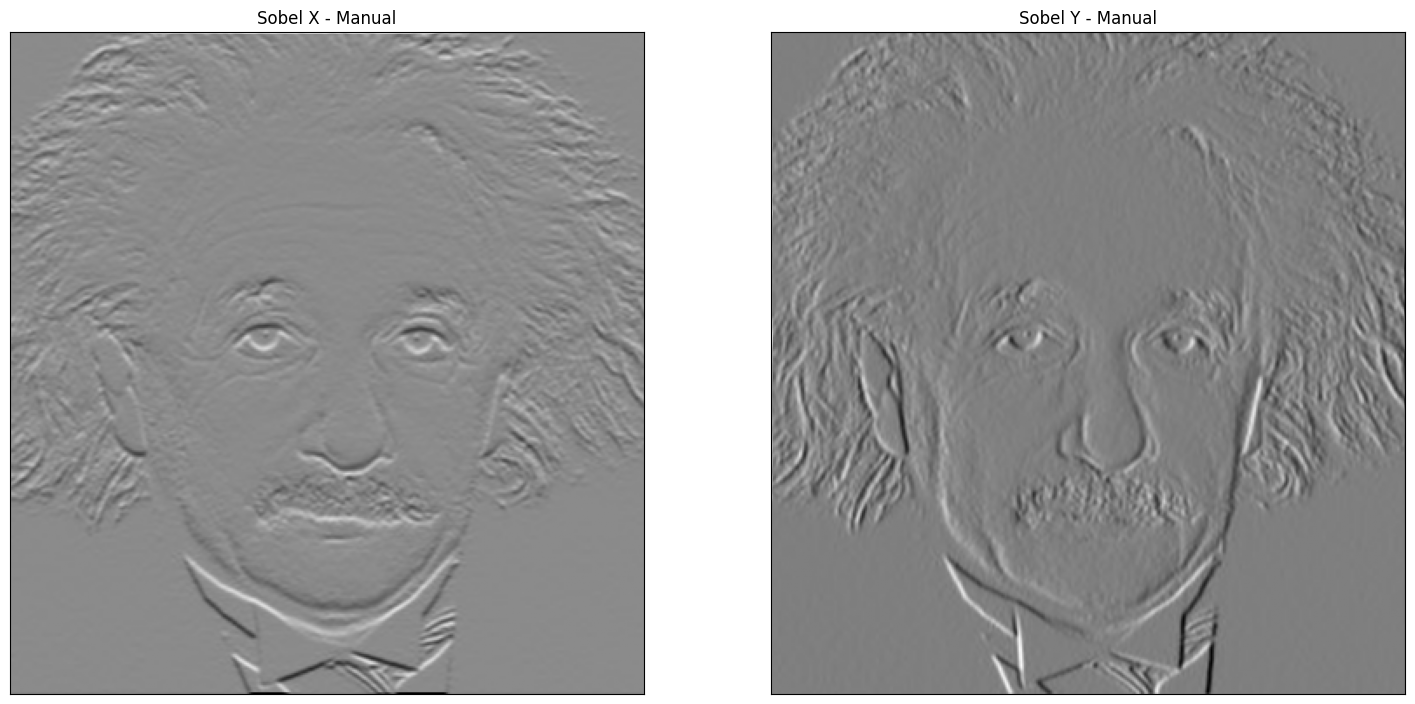
\includegraphics[width=0.65\linewidth]{resources/sobel_manual.png}
    \caption{Sobel Filtering}
    \label{fig:placeholder}
\end{figure}

\section*{Question 8: Image Zooming}
\subsubsection{Interpolation Methods}


\begin{lstlisting}[style=pythonstyle]
def zoom_image(img, target_size=None, scale=None, method="nearest"):
    if method == "nearest":
        interp = cv.INTER_NEAREST
    elif method == "bilinear":
        interp = cv.INTER_LINEAR

    if target_size is not None:
        return cv.resize(img, target_size, interpolation=interp)
    elif scale is not None and (0 < scale <= 10):
        h, w = img.shape[:2]
        return cv.resize(img, (int(w * scale), int(h * scale)), interpolation=interp)

def normalized_ssd(img1, img2):
    diff = img1.astype(np.float32) - img2.astype(np.float32)
    ssd = np.sum(diff ** 2)
    norm_ssd = ssd / np.sum(img1.astype(np.float32) ** 2)
    return norm_ssd
\end{lstlisting}

% \subsubsection*{Performance Evaluation}
% Normalized Sum of Squared Differences (SSD) calculations:
\begin{figure}[H]
    \centering
    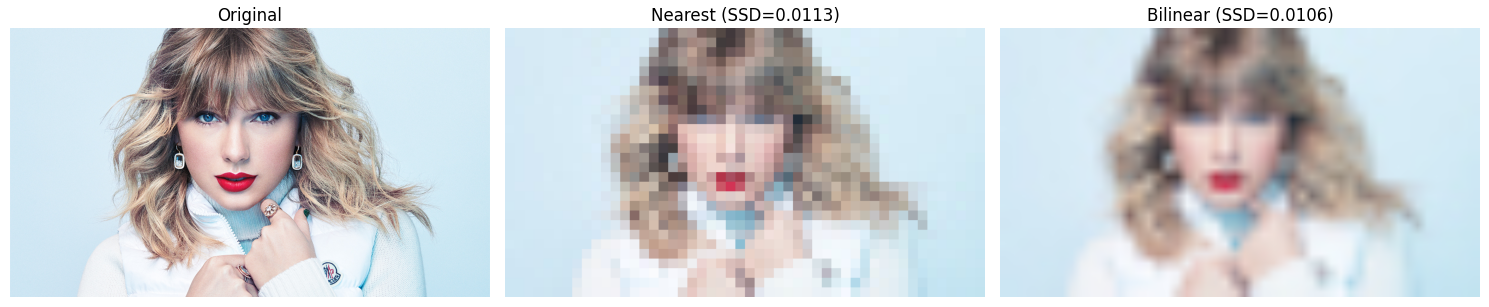
\includegraphics[width=0.9\linewidth]{resources/q8_taylor.png}
    %\caption{Caption}
    \label{fig:placeholder}
\end{figure}

\begin{figure}[H]
    \centering
    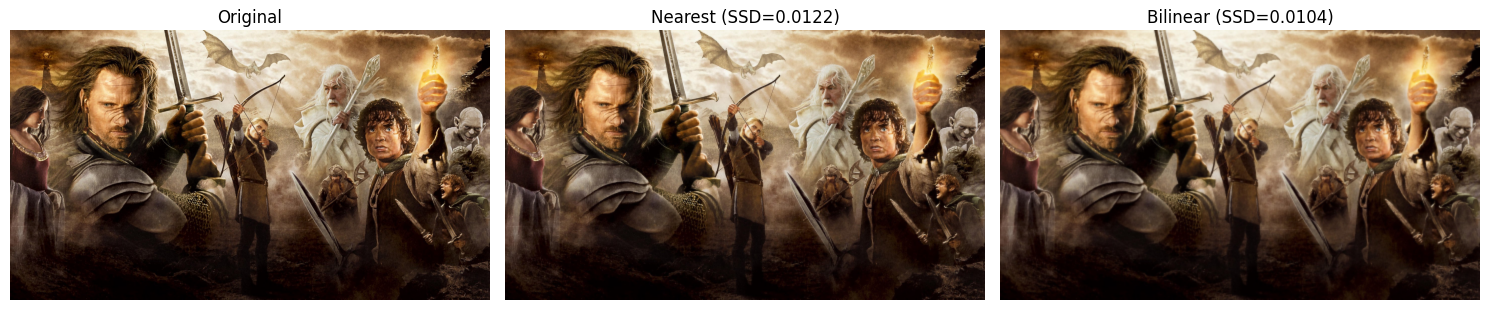
\includegraphics[width=0.9\linewidth]{resources/q8_king.png}
    %\caption{Caption}
    \label{fig:placeholder}
\end{figure}

\begin{figure}[H]
    \centering
    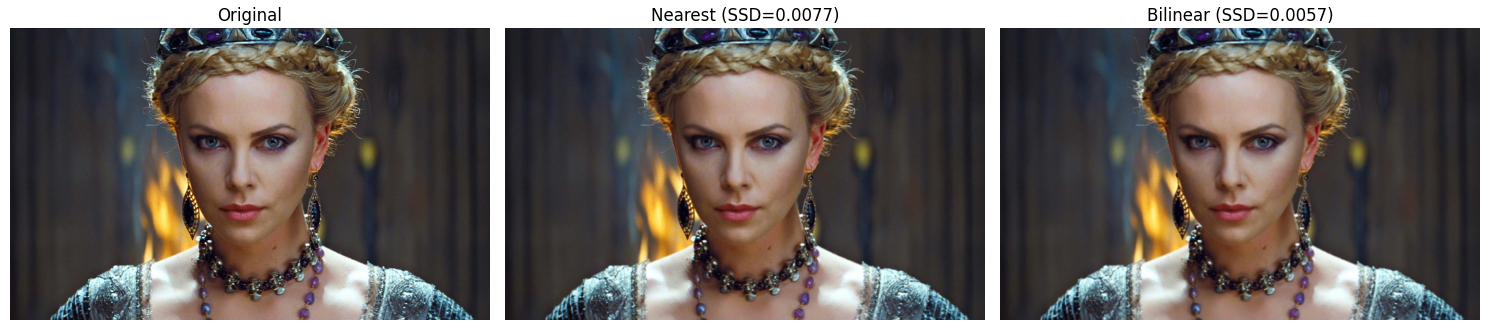
\includegraphics[width=0.9\linewidth]{resources/q8_queen.png}
    %\caption{Caption}
    \label{fig:placeholder}
\end{figure}


\subsubsection*{Results Analysis}
Bilinear interpolation produces smoother and more visually pleasing results compared to nearest neighbor. Additionally, the slightly lower SSD value for bilinear indicates a closer match to the reference image.


\section*{Question 9: Flower}
\begin{lstlisting}[style=pythonstyle]
mask = np.zeros(img.shape[:2], np.uint8)
bgdModel = np.zeros((1, 65), np.float64)
fgdModel = np.zeros((1, 65), np.float64)
rect = (50, 50, img.shape[1] - 50, img.shape[0] - 50)
# Run GrabCut
cv.grabCut(img_rgb, mask, rect, bgdModel, fgdModel, 5, cv.GC_INIT_WITH_RECT)
mask2 = np.where((mask == cv.GC_FGD) | (mask == cv.GC_PR_FGD), 1, 0).astype('uint8')
foreground = img_rgb * mask2[:, :, np.newaxis]
background = img_rgb * (1 - mask2[:, :, np.newaxis])
segmentation_mask = (mask2 * 255).astype(np.uint8)
# Blur the entire image
blurred = cv.GaussianBlur(img_rgb, (25, 25), 0)
enhanced = blurred.copy()
enhanced[mask2 == 1] = img_rgb[mask2 == 1]
\end{lstlisting}

\begin{figure}[H]
    \centering
    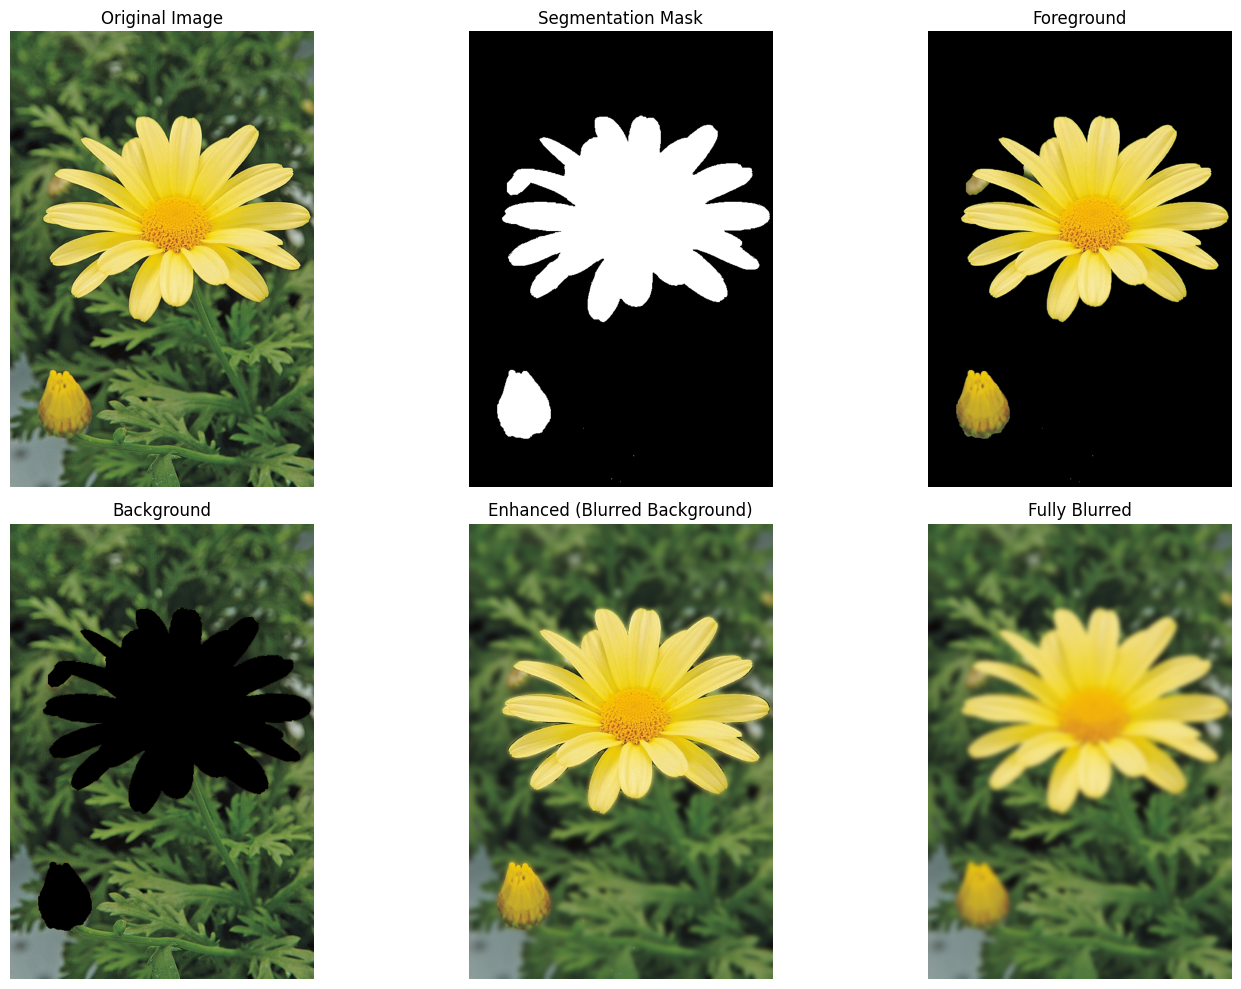
\includegraphics[width=0.8\linewidth]{resources/q9.png}
    %\caption{Caption}
    \label{fig:placeholder}
\end{figure}
\subsubsection*{Reason for dark background at flower edges}
When applying Gaussian blur to the background, the kernel averages surrounding pixels. Near the flower edges, some pixels are zeroed out from foreground extraction, causing the averaged values to be darker than the original background.
%%%%%%%%%%%%%%%%%%%%%%%%%%%%%%%%%%%%%%%%%%%%%%%%%%%%%%%%%%
% References
%%%%%%%%%%%%%%%%%%%%%%%%%%%%%%%%%%%%%%%%%%%%%%%%%%%%%%%%%%

% \newpage
% \addcontentsline{toc}{section}{References}
% \bibliographystyle{IEEEtran}
% \bibliography{references}

\end{document}

























